\documentclass[twoside]{book}

% Packages required by doxygen
\usepackage{fixltx2e}
\usepackage{calc}
\usepackage{doxygen}
\usepackage{graphicx}
\usepackage[utf8]{inputenc}
\usepackage{makeidx}
\usepackage{multicol}
\usepackage{multirow}
\PassOptionsToPackage{warn}{textcomp}
\usepackage{textcomp}
\usepackage[nointegrals]{wasysym}
\usepackage[table]{xcolor}

% Font selection
\usepackage[T1]{fontenc}
\usepackage{mathptmx}
\usepackage[scaled=.90]{helvet}
\usepackage{courier}
\usepackage{amssymb}
\usepackage{sectsty}
\renewcommand{\familydefault}{\sfdefault}
\allsectionsfont{%
  \fontseries{bc}\selectfont%
  \color{darkgray}%
}
\renewcommand{\DoxyLabelFont}{%
  \fontseries{bc}\selectfont%
  \color{darkgray}%
}
\newcommand{\+}{\discretionary{\mbox{\scriptsize$\hookleftarrow$}}{}{}}

% Page & text layout
\usepackage{geometry}
\geometry{%
  a4paper,%
  top=2.5cm,%
  bottom=2.5cm,%
  left=2.5cm,%
  right=2.5cm%
}
\tolerance=750
\hfuzz=15pt
\hbadness=750
\setlength{\emergencystretch}{15pt}
\setlength{\parindent}{0cm}
\setlength{\parskip}{0.2cm}
\makeatletter
\renewcommand{\paragraph}{%
  \@startsection{paragraph}{4}{0ex}{-1.0ex}{1.0ex}{%
    \normalfont\normalsize\bfseries\SS@parafont%
  }%
}
\renewcommand{\subparagraph}{%
  \@startsection{subparagraph}{5}{0ex}{-1.0ex}{1.0ex}{%
    \normalfont\normalsize\bfseries\SS@subparafont%
  }%
}
\makeatother

% Headers & footers
\usepackage{fancyhdr}
\pagestyle{fancyplain}
\fancyhead[LE]{\fancyplain{}{\bfseries\thepage}}
\fancyhead[CE]{\fancyplain{}{}}
\fancyhead[RE]{\fancyplain{}{\bfseries\leftmark}}
\fancyhead[LO]{\fancyplain{}{\bfseries\rightmark}}
\fancyhead[CO]{\fancyplain{}{}}
\fancyhead[RO]{\fancyplain{}{\bfseries\thepage}}
\fancyfoot[LE]{\fancyplain{}{}}
\fancyfoot[CE]{\fancyplain{}{}}
\fancyfoot[RE]{\fancyplain{}{\bfseries\scriptsize Generated on Fri Jun 5 2015 12\+:18\+:16 for S\+L\+O\+P\+E by Doxygen }}
\fancyfoot[LO]{\fancyplain{}{\bfseries\scriptsize Generated on Fri Jun 5 2015 12\+:18\+:16 for S\+L\+O\+P\+E by Doxygen }}
\fancyfoot[CO]{\fancyplain{}{}}
\fancyfoot[RO]{\fancyplain{}{}}
\renewcommand{\footrulewidth}{0.4pt}
\renewcommand{\chaptermark}[1]{%
  \markboth{#1}{}%
}
\renewcommand{\sectionmark}[1]{%
  \markright{\thesection\ #1}%
}

% Indices & bibliography
\usepackage{natbib}
\usepackage[titles]{tocloft}
\setcounter{tocdepth}{3}
\setcounter{secnumdepth}{5}
\makeindex

% Hyperlinks (required, but should be loaded last)
\usepackage{ifpdf}
\ifpdf
  \usepackage[pdftex,pagebackref=true]{hyperref}
\else
  \usepackage[ps2pdf,pagebackref=true]{hyperref}
\fi
\hypersetup{%
  colorlinks=true,%
  linkcolor=blue,%
  citecolor=blue,%
  unicode%
}

% Custom commands
\newcommand{\clearemptydoublepage}{%
  \newpage{\pagestyle{empty}\cleardoublepage}%
}


%===== C O N T E N T S =====

\begin{document}

% Titlepage & ToC
\hypersetup{pageanchor=false,
             bookmarks=true,
             bookmarksnumbered=true,
             pdfencoding=unicode
            }
\pagenumbering{roman}
\begin{titlepage}
\vspace*{7cm}
\begin{center}%
{\Large S\+L\+O\+P\+E }\\
\vspace*{1cm}
{\large Generated by Doxygen 1.8.8}\\
\vspace*{0.5cm}
{\small Fri Jun 5 2015 12:18:16}\\
\end{center}
\end{titlepage}
\clearemptydoublepage
\tableofcontents
\clearemptydoublepage
\pagenumbering{arabic}
\hypersetup{pageanchor=true}

%--- Begin generated contents ---
\chapter{Slope, a free charting library that uses cairo}
\label{index}\hypertarget{index}{}Slope is developed with the goal of providing an easy way to cairo and Gtk users to generate charts to visualize numerical data. The coding conventions are similar to those used in cairo.

Slope's only mandatory dependency is cairo, if you turn off the build flag that includes Gtk. The Gtk dependent build has the advantage of using the pango text layout library that is much more powerful than the cairo \char`\"{}toy\char`\"{} A\+P\+I for text rendering, and of course the ability to add a custom widget to your Gtk G\+U\+I with mouse zooming enabled. 
\chapter{S\+L\+O\+P\+E}
\label{md_README}
\hypertarget{md_README}{}
Slope is a free (L\+G\+P\+L) {\bfseries C} library that creates charts from numerical data. It's design principle is the following\+: {\bfseries T\+H\+E O\+N\+L\+Y D\+E\+P\+E\+N\+D\+E\+N\+C\+Y I\+S C\+A\+I\+R\+O}, and the {\bfseries A\+P\+I} is familiar to the users of cairo. Additionaly an alternative build provides a Gtk widget and some utilities so create simple chart windows and animations, such as real time data display. This build of course makes slope {\bfseries Gtk} dependent. The cairo only build will always be maintained.

Slope is in it's early stages of development and still needs some optimization and polishing. Some accessor methods to objects properties are also absent. But here's what we already have\+: The following chart is the output of the test.\+c program in de top level source repository.



Slope's basic usage is\+: create a {\bfseries slope\+\_\+figure\+\_\+t}, add one or more {\bfseries slope\+\_\+metrics\+\_\+t} to it and add some {\bfseries slope\+\_\+item\+\_\+t} to the metrics, then use function {\bfseries \hyperlink{group__Figure_ga386e261642ba2b0fdc39a550e3e94462}{slope\+\_\+figure\+\_\+draw()}} to stroke the resulting chart via a {\bfseries cairo\+\_\+t}.

Contributions to slope are welcome, propose your's to \href{mailto:elvismtt@gmail.com}{\tt elvismtt@gmail.\+com}

Special thanks to Remi Bertho (\href{mailto:remi.bertho@openmailbox.org}{\tt remi.\+bertho@openmailbox.\+org}) for his contributions 
\chapter{Module Index}
\section{Modules}
Here is a list of all modules\+:\begin{DoxyCompactList}
\item \contentsline{section}{Figure}{\pageref{group__Figure}}{}
\item \contentsline{section}{Item}{\pageref{group__Item}}{}
\item \contentsline{section}{List}{\pageref{group__List}}{}
\item \contentsline{section}{Metrics}{\pageref{group__Metrics}}{}
\item \contentsline{section}{Primitives}{\pageref{group__Primitives}}{}
\end{DoxyCompactList}

\chapter{Class Index}
\section{Class List}
Here are the classes, structs, unions and interfaces with brief descriptions\+:\begin{DoxyCompactList}
\item\contentsline{section}{\hyperlink{struct__slope__color}{\+\_\+slope\+\_\+color} }{\pageref{struct__slope__color}}{}
\item\contentsline{section}{\hyperlink{struct__slope__figure}{\+\_\+slope\+\_\+figure} }{\pageref{struct__slope__figure}}{}
\item\contentsline{section}{\hyperlink{struct__slope__item}{\+\_\+slope\+\_\+item} }{\pageref{struct__slope__item}}{}
\item\contentsline{section}{\hyperlink{struct__slope__item__class}{\+\_\+slope\+\_\+item\+\_\+class} }{\pageref{struct__slope__item__class}}{}
\item\contentsline{section}{\hyperlink{struct__slope__iterator}{\+\_\+slope\+\_\+iterator} }{\pageref{struct__slope__iterator}}{}
\item\contentsline{section}{\hyperlink{struct__slope__legend}{\+\_\+slope\+\_\+legend} }{\pageref{struct__slope__legend}}{}
\item\contentsline{section}{\hyperlink{struct__slope__list}{\+\_\+slope\+\_\+list} }{\pageref{struct__slope__list}}{}
\item\contentsline{section}{\hyperlink{struct__slope__metrics}{\+\_\+slope\+\_\+metrics} }{\pageref{struct__slope__metrics}}{}
\item\contentsline{section}{\hyperlink{struct__slope__metrics__class}{\+\_\+slope\+\_\+metrics\+\_\+class} }{\pageref{struct__slope__metrics__class}}{}
\item\contentsline{section}{\hyperlink{struct__slope__point}{\+\_\+slope\+\_\+point} }{\pageref{struct__slope__point}}{}
\item\contentsline{section}{\hyperlink{struct__slope__rect}{\+\_\+slope\+\_\+rect} }{\pageref{struct__slope__rect}}{}
\item\contentsline{section}{\hyperlink{struct__slope__vector}{\+\_\+slope\+\_\+vector} }{\pageref{struct__slope__vector}}{}
\item\contentsline{section}{\hyperlink{struct__slope__xyaxis}{\+\_\+slope\+\_\+xyaxis} }{\pageref{struct__slope__xyaxis}}{}
\item\contentsline{section}{\hyperlink{struct__slope__xyitem}{\+\_\+slope\+\_\+xyitem} }{\pageref{struct__slope__xyitem}}{}
\item\contentsline{section}{\hyperlink{struct__slope__xymetrics}{\+\_\+slope\+\_\+xymetrics} }{\pageref{struct__slope__xymetrics}}{}
\item\contentsline{section}{\hyperlink{struct__SlopeView}{\+\_\+\+Slope\+View} }{\pageref{struct__SlopeView}}{}
\item\contentsline{section}{\hyperlink{struct__SlopeViewClass}{\+\_\+\+Slope\+View\+Class} }{\pageref{struct__SlopeViewClass}}{}
\item\contentsline{section}{\hyperlink{struct__SlopeViewPrivate}{\+\_\+\+Slope\+View\+Private} }{\pageref{struct__SlopeViewPrivate}}{}
\end{DoxyCompactList}

\chapter{File Index}
\section{File List}
Here is a list of all documented files with brief descriptions\+:\begin{DoxyCompactList}
\item\contentsline{section}{slope/\hyperlink{figure_8h}{figure.\+h} }{\pageref{figure_8h}}{}
\item\contentsline{section}{slope/{\bfseries figure\+\_\+p.\+h} }{\pageref{figure__p_8h}}{}
\item\contentsline{section}{slope/{\bfseries global.\+h} }{\pageref{global_8h}}{}
\item\contentsline{section}{slope/{\bfseries gtk.\+h} }{\pageref{gtk_8h}}{}
\item\contentsline{section}{slope/\hyperlink{item_8h}{item.\+h} }{\pageref{item_8h}}{}
\item\contentsline{section}{slope/{\bfseries item\+\_\+p.\+h} }{\pageref{item__p_8h}}{}
\item\contentsline{section}{slope/{\bfseries legend.\+h} }{\pageref{legend_8h}}{}
\item\contentsline{section}{slope/{\bfseries legend\+\_\+p.\+h} }{\pageref{legend__p_8h}}{}
\item\contentsline{section}{slope/\hyperlink{list_8h}{list.\+h} }{\pageref{list_8h}}{}
\item\contentsline{section}{slope/\hyperlink{metrics_8h}{metrics.\+h} }{\pageref{metrics_8h}}{}
\item\contentsline{section}{slope/{\bfseries metrics\+\_\+p.\+h} }{\pageref{metrics__p_8h}}{}
\item\contentsline{section}{slope/\hyperlink{primitives_8h}{primitives.\+h} }{\pageref{primitives_8h}}{}
\item\contentsline{section}{slope/\hyperlink{slope_8h}{slope.\+h} }{\pageref{slope_8h}}{}
\item\contentsline{section}{slope/{\bfseries vector.\+h} }{\pageref{vector_8h}}{}
\item\contentsline{section}{slope/{\bfseries view.\+h} }{\pageref{view_8h}}{}
\item\contentsline{section}{slope/{\bfseries xyaxis.\+h} }{\pageref{xyaxis_8h}}{}
\item\contentsline{section}{slope/{\bfseries xyaxis\+\_\+p.\+h} }{\pageref{xyaxis__p_8h}}{}
\item\contentsline{section}{slope/{\bfseries xyitem.\+h} }{\pageref{xyitem_8h}}{}
\item\contentsline{section}{slope/{\bfseries xyitem\+\_\+p.\+h} }{\pageref{xyitem__p_8h}}{}
\item\contentsline{section}{slope/{\bfseries xymetrics.\+h} }{\pageref{xymetrics_8h}}{}
\item\contentsline{section}{slope/{\bfseries xymetrics\+\_\+p.\+h} }{\pageref{xymetrics__p_8h}}{}
\end{DoxyCompactList}

\chapter{Module Documentation}
\hypertarget{group__Figure}{\section{Figure}
\label{group__Figure}\index{Figure@{Figure}}
}


Figure is the object that holds any of slope's drawables.  


\subsection*{Typedefs}
\begin{DoxyCompactItemize}
\item 
\hypertarget{group__Figure_ga507cc82eeca8255d6c0f603ffdaeb59e}{typedef struct \hyperlink{struct__slope__figure}{\+\_\+slope\+\_\+figure} \hyperlink{group__Figure_ga507cc82eeca8255d6c0f603ffdaeb59e}{slope\+\_\+figure\+\_\+t}}\label{group__Figure_ga507cc82eeca8255d6c0f603ffdaeb59e}

\begin{DoxyCompactList}\small\item\em The figure type represents the final drawable of slopes architecture This is the final product os a user operation, it can dre drawn in any cairo backend like Gtk\+Widgets or one of many graphics file formats. \end{DoxyCompactList}\end{DoxyCompactItemize}
\subsection*{Functions}
\begin{DoxyCompactItemize}
\item 
S\+L\+O\+P\+E\+\_\+\+B\+E\+G\+I\+N\+\_\+\+D\+E\+C\+L\+S slope\+\_\+public \\*
\hyperlink{group__Figure_ga507cc82eeca8255d6c0f603ffdaeb59e}{slope\+\_\+figure\+\_\+t} $\ast$ \hyperlink{group__Figure_ga0534b5fef88fda65fd4b8feb33071cab}{slope\+\_\+figure\+\_\+create} ()
\begin{DoxyCompactList}\small\item\em Creates a new figure object. \end{DoxyCompactList}\item 
slope\+\_\+public \hyperlink{struct__slope__list}{slope\+\_\+list\+\_\+t} $\ast$ \hyperlink{group__Figure_gac7d6aaca4df6806f00f3cb130a78dcde}{slope\+\_\+figure\+\_\+get\+\_\+metrics\+\_\+list} (const \hyperlink{group__Figure_ga507cc82eeca8255d6c0f603ffdaeb59e}{slope\+\_\+figure\+\_\+t} $\ast$figure)
\begin{DoxyCompactList}\small\item\em Retrieves the metrics list of figure. \end{DoxyCompactList}\item 
\hypertarget{group__Figure_ga08b6896169ef4a926e7d487ade3fe74e}{slope\+\_\+public void \hyperlink{group__Figure_ga08b6896169ef4a926e7d487ade3fe74e}{slope\+\_\+figure\+\_\+add\+\_\+metrics} (\hyperlink{group__Figure_ga507cc82eeca8255d6c0f603ffdaeb59e}{slope\+\_\+figure\+\_\+t} $\ast$figure, \hyperlink{group__Metrics_gab80787ee8ae8dc449e770249fe0e3c35}{slope\+\_\+metrics\+\_\+t} $\ast$metrics)}\label{group__Figure_ga08b6896169ef4a926e7d487ade3fe74e}

\begin{DoxyCompactList}\small\item\em Adds a metrics the metrics list of figure. \end{DoxyCompactList}\item 
\hypertarget{group__Figure_gada369b301fabc0c40ef172e22d4fcb85}{slope\+\_\+public void \hyperlink{group__Figure_gada369b301fabc0c40ef172e22d4fcb85}{slope\+\_\+figure\+\_\+destroy} (\hyperlink{group__Figure_ga507cc82eeca8255d6c0f603ffdaeb59e}{slope\+\_\+figure\+\_\+t} $\ast$figure)}\label{group__Figure_gada369b301fabc0c40ef172e22d4fcb85}

\begin{DoxyCompactList}\small\item\em Destroys any figure object and frees the memory used by it. \end{DoxyCompactList}\item 
slope\+\_\+public void \hyperlink{group__Figure_ga386e261642ba2b0fdc39a550e3e94462}{slope\+\_\+figure\+\_\+draw} (\hyperlink{group__Figure_ga507cc82eeca8255d6c0f603ffdaeb59e}{slope\+\_\+figure\+\_\+t} $\ast$figure, cairo\+\_\+t $\ast$cr, const \hyperlink{struct__slope__rect}{slope\+\_\+rect\+\_\+t} $\ast$rect)
\begin{DoxyCompactList}\small\item\em Draw the contents of this figure to one of cairo's backends via cr. \end{DoxyCompactList}\item 
slope\+\_\+public void \hyperlink{group__Figure_ga586a40d60b3c5feec3f74f1bb00b011d}{slope\+\_\+figure\+\_\+write\+\_\+to\+\_\+png} (\hyperlink{group__Figure_ga507cc82eeca8255d6c0f603ffdaeb59e}{slope\+\_\+figure\+\_\+t} $\ast$figure, const char $\ast$filename, int width, int height)
\begin{DoxyCompactList}\small\item\em Writes the figure to a png file. \end{DoxyCompactList}\item 
slope\+\_\+public int \hyperlink{group__Figure_ga18b13f5d94a871984760eaa4b5f5f4ae}{slope\+\_\+figure\+\_\+write\+\_\+to\+\_\+svg} (\hyperlink{group__Figure_ga507cc82eeca8255d6c0f603ffdaeb59e}{slope\+\_\+figure\+\_\+t} $\ast$figure, const char $\ast$filename, int width, int height)
\begin{DoxyCompactList}\small\item\em The figure to be drawn. \end{DoxyCompactList}\item 
slope\+\_\+public int \hyperlink{group__Figure_ga3d70896b8765c2ea7058e5213daa17fd}{slope\+\_\+figure\+\_\+write\+\_\+to\+\_\+pdf} (\hyperlink{group__Figure_ga507cc82eeca8255d6c0f603ffdaeb59e}{slope\+\_\+figure\+\_\+t} $\ast$figure, const char $\ast$filename, int width, int height)
\begin{DoxyCompactList}\small\item\em The figure to be drawn. \end{DoxyCompactList}\item 
slope\+\_\+public int \hyperlink{group__Figure_gaad033abcd87cdbae258f073c6f43101b}{slope\+\_\+figure\+\_\+write\+\_\+to\+\_\+ps} (\hyperlink{group__Figure_ga507cc82eeca8255d6c0f603ffdaeb59e}{slope\+\_\+figure\+\_\+t} $\ast$figure, const char $\ast$filename, int width, int height)
\begin{DoxyCompactList}\small\item\em The figure to be drawn. \end{DoxyCompactList}\item 
slope\+\_\+public \hyperlink{group__Metrics_gab80787ee8ae8dc449e770249fe0e3c35}{slope\+\_\+metrics\+\_\+t} $\ast$ \hyperlink{group__Figure_gae97736e589280dfdd5446500c576887a}{slope\+\_\+figure\+\_\+get\+\_\+default\+\_\+metrics} (\hyperlink{group__Figure_ga507cc82eeca8255d6c0f603ffdaeb59e}{slope\+\_\+figure\+\_\+t} $\ast$figure)
\begin{DoxyCompactList}\small\item\em Retrieves the default metrics of the figure, normaly the last to be inserted. It is the one that will place the legend. \end{DoxyCompactList}\item 
slope\+\_\+public void \hyperlink{group__Figure_gad9907caa20c827f090b140e389f3c077}{slope\+\_\+figure\+\_\+set\+\_\+change\+\_\+callback} (\hyperlink{group__Figure_ga507cc82eeca8255d6c0f603ffdaeb59e}{slope\+\_\+figure\+\_\+t} $\ast$figure, slope\+\_\+callback\+\_\+t callback)
\begin{DoxyCompactList}\small\item\em Sets a callback to be called when some thing change on the figure, e. g. useful to tell a widget to update it1s contents. \end{DoxyCompactList}\end{DoxyCompactItemize}


\subsection{Detailed Description}
Figure is the object that holds any of slope's drawables. 

Every time one wants to produce a figure one will instantiate a slope\+\_\+figure\+\_\+t, add one or more slope\+\_\+metrics\+\_\+t to it and then place the slope\+\_\+item\+\_\+t's in the metrics. All that remains to do is draw the figure to any of cairo's backends, such as a Gtk\+Widget a P\+N\+G file or any other. 

\subsection{Function Documentation}
\hypertarget{group__Figure_ga0534b5fef88fda65fd4b8feb33071cab}{\index{Figure@{Figure}!slope\+\_\+figure\+\_\+create@{slope\+\_\+figure\+\_\+create}}
\index{slope\+\_\+figure\+\_\+create@{slope\+\_\+figure\+\_\+create}!Figure@{Figure}}
\subsubsection[{slope\+\_\+figure\+\_\+create}]{\setlength{\rightskip}{0pt plus 5cm}S\+L\+O\+P\+E\+\_\+\+B\+E\+G\+I\+N\+\_\+\+D\+E\+C\+L\+S slope\+\_\+public {\bf slope\+\_\+figure\+\_\+t}$\ast$ slope\+\_\+figure\+\_\+create (
\begin{DoxyParamCaption}
{}
\end{DoxyParamCaption}
)}}\label{group__Figure_ga0534b5fef88fda65fd4b8feb33071cab}


Creates a new figure object. 

\begin{DoxyReturn}{Returns}
A new figure instance. 
\end{DoxyReturn}
\hypertarget{group__Figure_ga386e261642ba2b0fdc39a550e3e94462}{\index{Figure@{Figure}!slope\+\_\+figure\+\_\+draw@{slope\+\_\+figure\+\_\+draw}}
\index{slope\+\_\+figure\+\_\+draw@{slope\+\_\+figure\+\_\+draw}!Figure@{Figure}}
\subsubsection[{slope\+\_\+figure\+\_\+draw}]{\setlength{\rightskip}{0pt plus 5cm}slope\+\_\+public void slope\+\_\+figure\+\_\+draw (
\begin{DoxyParamCaption}
\item[{{\bf slope\+\_\+figure\+\_\+t} $\ast$}]{figure, }
\item[{cairo\+\_\+t $\ast$}]{cr, }
\item[{const {\bf slope\+\_\+rect\+\_\+t} $\ast$}]{rect}
\end{DoxyParamCaption}
)}}\label{group__Figure_ga386e261642ba2b0fdc39a550e3e94462}


Draw the contents of this figure to one of cairo's backends via cr. 


\begin{DoxyParams}{Parameters}
{\em figure} & The figure to be drawn. \\
\hline
{\em cr} & The cairo context to draw the figure. \\
\hline
{\em rect} & The rectange that limits the area of the cairo\+\_\+surface\+\_\+t to draw figure. \\
\hline
\end{DoxyParams}
\hypertarget{group__Figure_gae97736e589280dfdd5446500c576887a}{\index{Figure@{Figure}!slope\+\_\+figure\+\_\+get\+\_\+default\+\_\+metrics@{slope\+\_\+figure\+\_\+get\+\_\+default\+\_\+metrics}}
\index{slope\+\_\+figure\+\_\+get\+\_\+default\+\_\+metrics@{slope\+\_\+figure\+\_\+get\+\_\+default\+\_\+metrics}!Figure@{Figure}}
\subsubsection[{slope\+\_\+figure\+\_\+get\+\_\+default\+\_\+metrics}]{\setlength{\rightskip}{0pt plus 5cm}slope\+\_\+public {\bf slope\+\_\+metrics\+\_\+t}$\ast$ slope\+\_\+figure\+\_\+get\+\_\+default\+\_\+metrics (
\begin{DoxyParamCaption}
\item[{{\bf slope\+\_\+figure\+\_\+t} $\ast$}]{figure}
\end{DoxyParamCaption}
)}}\label{group__Figure_gae97736e589280dfdd5446500c576887a}


Retrieves the default metrics of the figure, normaly the last to be inserted. It is the one that will place the legend. 


\begin{DoxyParams}{Parameters}
{\em figure} & The figure from wich to get the default metrics.\\
\hline
\end{DoxyParams}
\begin{DoxyReturn}{Returns}
A pointer default metrics of figure. 
\end{DoxyReturn}
\hypertarget{group__Figure_gac7d6aaca4df6806f00f3cb130a78dcde}{\index{Figure@{Figure}!slope\+\_\+figure\+\_\+get\+\_\+metrics\+\_\+list@{slope\+\_\+figure\+\_\+get\+\_\+metrics\+\_\+list}}
\index{slope\+\_\+figure\+\_\+get\+\_\+metrics\+\_\+list@{slope\+\_\+figure\+\_\+get\+\_\+metrics\+\_\+list}!Figure@{Figure}}
\subsubsection[{slope\+\_\+figure\+\_\+get\+\_\+metrics\+\_\+list}]{\setlength{\rightskip}{0pt plus 5cm}slope\+\_\+public {\bf slope\+\_\+list\+\_\+t}$\ast$ slope\+\_\+figure\+\_\+get\+\_\+metrics\+\_\+list (
\begin{DoxyParamCaption}
\item[{const {\bf slope\+\_\+figure\+\_\+t} $\ast$}]{figure}
\end{DoxyParamCaption}
)}}\label{group__Figure_gac7d6aaca4df6806f00f3cb130a78dcde}


Retrieves the metrics list of figure. 

\begin{DoxyReturn}{Returns}
The list of metrics in this figure. 
\end{DoxyReturn}
\hypertarget{group__Figure_gad9907caa20c827f090b140e389f3c077}{\index{Figure@{Figure}!slope\+\_\+figure\+\_\+set\+\_\+change\+\_\+callback@{slope\+\_\+figure\+\_\+set\+\_\+change\+\_\+callback}}
\index{slope\+\_\+figure\+\_\+set\+\_\+change\+\_\+callback@{slope\+\_\+figure\+\_\+set\+\_\+change\+\_\+callback}!Figure@{Figure}}
\subsubsection[{slope\+\_\+figure\+\_\+set\+\_\+change\+\_\+callback}]{\setlength{\rightskip}{0pt plus 5cm}slope\+\_\+public void slope\+\_\+figure\+\_\+set\+\_\+change\+\_\+callback (
\begin{DoxyParamCaption}
\item[{{\bf slope\+\_\+figure\+\_\+t} $\ast$}]{figure, }
\item[{slope\+\_\+callback\+\_\+t}]{callback}
\end{DoxyParamCaption}
)}}\label{group__Figure_gad9907caa20c827f090b140e389f3c077}


Sets a callback to be called when some thing change on the figure, e. g. useful to tell a widget to update it1s contents. 


\begin{DoxyParams}{Parameters}
{\em figure} & The figure in which some thing changed \\
\hline
{\em callback} & A pointer to a function to be called when figure changes \\
\hline
\end{DoxyParams}
\hypertarget{group__Figure_ga3d70896b8765c2ea7058e5213daa17fd}{\index{Figure@{Figure}!slope\+\_\+figure\+\_\+write\+\_\+to\+\_\+pdf@{slope\+\_\+figure\+\_\+write\+\_\+to\+\_\+pdf}}
\index{slope\+\_\+figure\+\_\+write\+\_\+to\+\_\+pdf@{slope\+\_\+figure\+\_\+write\+\_\+to\+\_\+pdf}!Figure@{Figure}}
\subsubsection[{slope\+\_\+figure\+\_\+write\+\_\+to\+\_\+pdf}]{\setlength{\rightskip}{0pt plus 5cm}slope\+\_\+public int slope\+\_\+figure\+\_\+write\+\_\+to\+\_\+pdf (
\begin{DoxyParamCaption}
\item[{{\bf slope\+\_\+figure\+\_\+t} $\ast$}]{figure, }
\item[{const char $\ast$}]{filename, }
\item[{int}]{width, }
\item[{int}]{height}
\end{DoxyParamCaption}
)}}\label{group__Figure_ga3d70896b8765c2ea7058e5213daa17fd}


The figure to be drawn. 


\begin{DoxyParams}{Parameters}
{\em figure} & The figure to be drawn \\
\hline
{\em filename} & The path to the pdf file to be output, include the .pdf ending. \\
\hline
{\em width} & The width in pixels of the output file. \\
\hline
{\em height} & The height in pixels of the output file.\\
\hline
\end{DoxyParams}
\begin{DoxyReturn}{Returns}
The status of the operation 
\end{DoxyReturn}
\hypertarget{group__Figure_ga586a40d60b3c5feec3f74f1bb00b011d}{\index{Figure@{Figure}!slope\+\_\+figure\+\_\+write\+\_\+to\+\_\+png@{slope\+\_\+figure\+\_\+write\+\_\+to\+\_\+png}}
\index{slope\+\_\+figure\+\_\+write\+\_\+to\+\_\+png@{slope\+\_\+figure\+\_\+write\+\_\+to\+\_\+png}!Figure@{Figure}}
\subsubsection[{slope\+\_\+figure\+\_\+write\+\_\+to\+\_\+png}]{\setlength{\rightskip}{0pt plus 5cm}slope\+\_\+public void slope\+\_\+figure\+\_\+write\+\_\+to\+\_\+png (
\begin{DoxyParamCaption}
\item[{{\bf slope\+\_\+figure\+\_\+t} $\ast$}]{figure, }
\item[{const char $\ast$}]{filename, }
\item[{int}]{width, }
\item[{int}]{height}
\end{DoxyParamCaption}
)}}\label{group__Figure_ga586a40d60b3c5feec3f74f1bb00b011d}


Writes the figure to a png file. 


\begin{DoxyParams}{Parameters}
{\em figure} & The figure to be drawn \\
\hline
{\em The} & figure to be drawn. \\
\hline
{\em filename} & The path to the png file to be output, include the .png ending. \\
\hline
{\em width} & The width in pixels of the output file. \\
\hline
{\em height} & The height in pixels of the output file. \\
\hline
\end{DoxyParams}
\hypertarget{group__Figure_gaad033abcd87cdbae258f073c6f43101b}{\index{Figure@{Figure}!slope\+\_\+figure\+\_\+write\+\_\+to\+\_\+ps@{slope\+\_\+figure\+\_\+write\+\_\+to\+\_\+ps}}
\index{slope\+\_\+figure\+\_\+write\+\_\+to\+\_\+ps@{slope\+\_\+figure\+\_\+write\+\_\+to\+\_\+ps}!Figure@{Figure}}
\subsubsection[{slope\+\_\+figure\+\_\+write\+\_\+to\+\_\+ps}]{\setlength{\rightskip}{0pt plus 5cm}slope\+\_\+public int slope\+\_\+figure\+\_\+write\+\_\+to\+\_\+ps (
\begin{DoxyParamCaption}
\item[{{\bf slope\+\_\+figure\+\_\+t} $\ast$}]{figure, }
\item[{const char $\ast$}]{filename, }
\item[{int}]{width, }
\item[{int}]{height}
\end{DoxyParamCaption}
)}}\label{group__Figure_gaad033abcd87cdbae258f073c6f43101b}


The figure to be drawn. 


\begin{DoxyParams}{Parameters}
{\em figure} & The figure to be drawn \\
\hline
{\em filename} & The path to the postscript file to be output, include the .ps ending. \\
\hline
{\em width} & The width in pixels of the output file. \\
\hline
{\em height} & The height in pixels of the output file.\\
\hline
\end{DoxyParams}
\begin{DoxyReturn}{Returns}
The status of the operation 
\end{DoxyReturn}
\hypertarget{group__Figure_ga18b13f5d94a871984760eaa4b5f5f4ae}{\index{Figure@{Figure}!slope\+\_\+figure\+\_\+write\+\_\+to\+\_\+svg@{slope\+\_\+figure\+\_\+write\+\_\+to\+\_\+svg}}
\index{slope\+\_\+figure\+\_\+write\+\_\+to\+\_\+svg@{slope\+\_\+figure\+\_\+write\+\_\+to\+\_\+svg}!Figure@{Figure}}
\subsubsection[{slope\+\_\+figure\+\_\+write\+\_\+to\+\_\+svg}]{\setlength{\rightskip}{0pt plus 5cm}slope\+\_\+public int slope\+\_\+figure\+\_\+write\+\_\+to\+\_\+svg (
\begin{DoxyParamCaption}
\item[{{\bf slope\+\_\+figure\+\_\+t} $\ast$}]{figure, }
\item[{const char $\ast$}]{filename, }
\item[{int}]{width, }
\item[{int}]{height}
\end{DoxyParamCaption}
)}}\label{group__Figure_ga18b13f5d94a871984760eaa4b5f5f4ae}


The figure to be drawn. 


\begin{DoxyParams}{Parameters}
{\em figure} & The figure to be drawn \\
\hline
{\em filename} & The path to the svg file to be output, include the .svg ending. \\
\hline
{\em width} & The width in pixels of the output file. \\
\hline
{\em height} & The height in pixels of the output file.\\
\hline
\end{DoxyParams}
\begin{DoxyReturn}{Returns}
The status of the operation 
\end{DoxyReturn}

\hypertarget{group__Item}{\section{Item}
\label{group__Item}\index{Item@{Item}}
}


The base class for item objects.  


\subsection*{Typedefs}
\begin{DoxyCompactItemize}
\item 
\hypertarget{group__Item_ga2616141f0e164a876049da51ea3a8646}{typedef struct \hyperlink{struct__slope__item}{\+\_\+slope\+\_\+item} \hyperlink{group__Item_ga2616141f0e164a876049da51ea3a8646}{slope\+\_\+item\+\_\+t}}\label{group__Item_ga2616141f0e164a876049da51ea3a8646}

\begin{DoxyCompactList}\small\item\em Every thing that can be drawn to a figure is a subclass of slope\+\_\+item\+\_\+t. \end{DoxyCompactList}\end{DoxyCompactItemize}
\subsection*{Enumerations}
\begin{DoxyCompactItemize}
\item 
enum \hyperlink{group__Item_ga7be66725a3a198bcbd9434e6d3ad70c5}{slope\+\_\+scatter\+\_\+t} \{ \\*
\hyperlink{group__Item_gga7be66725a3a198bcbd9434e6d3ad70c5a54cf36614caf64fac788937a888664d7}{S\+L\+O\+P\+E\+\_\+\+L\+I\+N\+E} = 0, 
\hyperlink{group__Item_gga7be66725a3a198bcbd9434e6d3ad70c5ad80e96cfe8b1fc4e166a9dd2916949a9}{S\+L\+O\+P\+E\+\_\+\+C\+I\+R\+C\+L\+E\+S} = 1, 
\hyperlink{group__Item_gga7be66725a3a198bcbd9434e6d3ad70c5a49e3d5b6cb489463f001bdf14d484315}{S\+L\+O\+P\+E\+\_\+\+T\+R\+I\+A\+N\+G\+L\+E\+S} = 2, 
\hyperlink{group__Item_gga7be66725a3a198bcbd9434e6d3ad70c5a5f482758196621c2a65e206ef287f030}{S\+L\+O\+P\+E\+\_\+\+S\+Q\+U\+A\+R\+E\+S} = 3, 
\\*
\hyperlink{group__Item_gga7be66725a3a198bcbd9434e6d3ad70c5a9eb209c97e09aa4121f056641c60e56c}{S\+L\+O\+P\+E\+\_\+\+P\+L\+U\+S\+S\+E\+S} = 4
 \}
\begin{DoxyCompactList}\small\item\em The symbol to represent a data point in a scatter map type chart. \end{DoxyCompactList}\end{DoxyCompactItemize}
\subsection*{Functions}
\begin{DoxyCompactItemize}
\item 
slope\+\_\+public void \hyperlink{group__Item_gaf048bd8c425893229133befa61831fd6}{slope\+\_\+item\+\_\+destroy} (\hyperlink{group__Item_ga2616141f0e164a876049da51ea3a8646}{slope\+\_\+item\+\_\+t} $\ast$item)
\begin{DoxyCompactList}\small\item\em Destroys an item and frees the memory. \end{DoxyCompactList}\item 
slope\+\_\+public int \hyperlink{group__Item_gaf9e09ab9591e1a2c3c41441f206ffd38}{slope\+\_\+item\+\_\+get\+\_\+visible} (const \hyperlink{group__Item_ga2616141f0e164a876049da51ea3a8646}{slope\+\_\+item\+\_\+t} $\ast$item)
\begin{DoxyCompactList}\small\item\em Queries for the visibility of an item. \end{DoxyCompactList}\item 
\hypertarget{group__Item_ga68b3c890dee408f284bb9c243b9dd0e9}{slope\+\_\+public void \hyperlink{group__Item_ga68b3c890dee408f284bb9c243b9dd0e9}{slope\+\_\+item\+\_\+toggle\+\_\+visible} (\hyperlink{group__Item_ga2616141f0e164a876049da51ea3a8646}{slope\+\_\+item\+\_\+t} $\ast$item, \hyperlink{group__Primitives_gac55afa016ca777119a6c343d1655d558}{slope\+\_\+bool\+\_\+t} visible)}\label{group__Item_ga68b3c890dee408f284bb9c243b9dd0e9}

\begin{DoxyCompactList}\small\item\em Sets the visibility state of the item. \end{DoxyCompactList}\end{DoxyCompactItemize}


\subsection{Detailed Description}
The base class for item objects. 

\begin{DoxyAuthor}{Author}
Elvis Teixeira 
\end{DoxyAuthor}
\begin{DoxyDate}{Date}
18 Jan 2015
\end{DoxyDate}
Everithing that can be drawn in a slope\+\_\+figure\+\_\+t, including data representations, chart axis, legends and text labels, are items. To be drawn, items must lie in the item list of metrics that that lie in the metrics list of a figure. 

\subsection{Enumeration Type Documentation}
\hypertarget{group__Item_ga7be66725a3a198bcbd9434e6d3ad70c5}{\index{Item@{Item}!slope\+\_\+scatter\+\_\+t@{slope\+\_\+scatter\+\_\+t}}
\index{slope\+\_\+scatter\+\_\+t@{slope\+\_\+scatter\+\_\+t}!Item@{Item}}
\subsubsection[{slope\+\_\+scatter\+\_\+t}]{\setlength{\rightskip}{0pt plus 5cm}enum {\bf slope\+\_\+scatter\+\_\+t}}}\label{group__Item_ga7be66725a3a198bcbd9434e6d3ad70c5}


The symbol to represent a data point in a scatter map type chart. 

\begin{Desc}
\item[Enumerator]\par
\begin{description}
\index{S\+L\+O\+P\+E\+\_\+\+L\+I\+N\+E@{S\+L\+O\+P\+E\+\_\+\+L\+I\+N\+E}!Item@{Item}}\index{Item@{Item}!S\+L\+O\+P\+E\+\_\+\+L\+I\+N\+E@{S\+L\+O\+P\+E\+\_\+\+L\+I\+N\+E}}\item[{\em 
\hypertarget{group__Item_gga7be66725a3a198bcbd9434e6d3ad70c5a54cf36614caf64fac788937a888664d7}{S\+L\+O\+P\+E\+\_\+\+L\+I\+N\+E}\label{group__Item_gga7be66725a3a198bcbd9434e6d3ad70c5a54cf36614caf64fac788937a888664d7}
}]The data points are joined by lines \index{S\+L\+O\+P\+E\+\_\+\+C\+I\+R\+C\+L\+E\+S@{S\+L\+O\+P\+E\+\_\+\+C\+I\+R\+C\+L\+E\+S}!Item@{Item}}\index{Item@{Item}!S\+L\+O\+P\+E\+\_\+\+C\+I\+R\+C\+L\+E\+S@{S\+L\+O\+P\+E\+\_\+\+C\+I\+R\+C\+L\+E\+S}}\item[{\em 
\hypertarget{group__Item_gga7be66725a3a198bcbd9434e6d3ad70c5ad80e96cfe8b1fc4e166a9dd2916949a9}{S\+L\+O\+P\+E\+\_\+\+C\+I\+R\+C\+L\+E\+S}\label{group__Item_gga7be66725a3a198bcbd9434e6d3ad70c5ad80e96cfe8b1fc4e166a9dd2916949a9}
}]The data points are represent by circles, filled or not \index{S\+L\+O\+P\+E\+\_\+\+T\+R\+I\+A\+N\+G\+L\+E\+S@{S\+L\+O\+P\+E\+\_\+\+T\+R\+I\+A\+N\+G\+L\+E\+S}!Item@{Item}}\index{Item@{Item}!S\+L\+O\+P\+E\+\_\+\+T\+R\+I\+A\+N\+G\+L\+E\+S@{S\+L\+O\+P\+E\+\_\+\+T\+R\+I\+A\+N\+G\+L\+E\+S}}\item[{\em 
\hypertarget{group__Item_gga7be66725a3a198bcbd9434e6d3ad70c5a49e3d5b6cb489463f001bdf14d484315}{S\+L\+O\+P\+E\+\_\+\+T\+R\+I\+A\+N\+G\+L\+E\+S}\label{group__Item_gga7be66725a3a198bcbd9434e6d3ad70c5a49e3d5b6cb489463f001bdf14d484315}
}]The data points are represent by triangles, filled or not \index{S\+L\+O\+P\+E\+\_\+\+S\+Q\+U\+A\+R\+E\+S@{S\+L\+O\+P\+E\+\_\+\+S\+Q\+U\+A\+R\+E\+S}!Item@{Item}}\index{Item@{Item}!S\+L\+O\+P\+E\+\_\+\+S\+Q\+U\+A\+R\+E\+S@{S\+L\+O\+P\+E\+\_\+\+S\+Q\+U\+A\+R\+E\+S}}\item[{\em 
\hypertarget{group__Item_gga7be66725a3a198bcbd9434e6d3ad70c5a5f482758196621c2a65e206ef287f030}{S\+L\+O\+P\+E\+\_\+\+S\+Q\+U\+A\+R\+E\+S}\label{group__Item_gga7be66725a3a198bcbd9434e6d3ad70c5a5f482758196621c2a65e206ef287f030}
}]The data points are represent by squares, filled or not \index{S\+L\+O\+P\+E\+\_\+\+P\+L\+U\+S\+S\+E\+S@{S\+L\+O\+P\+E\+\_\+\+P\+L\+U\+S\+S\+E\+S}!Item@{Item}}\index{Item@{Item}!S\+L\+O\+P\+E\+\_\+\+P\+L\+U\+S\+S\+E\+S@{S\+L\+O\+P\+E\+\_\+\+P\+L\+U\+S\+S\+E\+S}}\item[{\em 
\hypertarget{group__Item_gga7be66725a3a198bcbd9434e6d3ad70c5a9eb209c97e09aa4121f056641c60e56c}{S\+L\+O\+P\+E\+\_\+\+P\+L\+U\+S\+S\+E\+S}\label{group__Item_gga7be66725a3a198bcbd9434e6d3ad70c5a9eb209c97e09aa4121f056641c60e56c}
}]The data points are represent by plus signs \end{description}
\end{Desc}


\subsection{Function Documentation}
\hypertarget{group__Item_gaf048bd8c425893229133befa61831fd6}{\index{Item@{Item}!slope\+\_\+item\+\_\+destroy@{slope\+\_\+item\+\_\+destroy}}
\index{slope\+\_\+item\+\_\+destroy@{slope\+\_\+item\+\_\+destroy}!Item@{Item}}
\subsubsection[{slope\+\_\+item\+\_\+destroy}]{\setlength{\rightskip}{0pt plus 5cm}slope\+\_\+public void slope\+\_\+item\+\_\+destroy (
\begin{DoxyParamCaption}
\item[{{\bf slope\+\_\+item\+\_\+t} $\ast$}]{item}
\end{DoxyParamCaption}
)}}\label{group__Item_gaf048bd8c425893229133befa61831fd6}


Destroys an item and frees the memory. 


\begin{DoxyParams}[1]{Parameters}
\mbox{\tt in}  & {\em item} & The item to be destroyed. \\
\hline
\end{DoxyParams}
\hypertarget{group__Item_gaf9e09ab9591e1a2c3c41441f206ffd38}{\index{Item@{Item}!slope\+\_\+item\+\_\+get\+\_\+visible@{slope\+\_\+item\+\_\+get\+\_\+visible}}
\index{slope\+\_\+item\+\_\+get\+\_\+visible@{slope\+\_\+item\+\_\+get\+\_\+visible}!Item@{Item}}
\subsubsection[{slope\+\_\+item\+\_\+get\+\_\+visible}]{\setlength{\rightskip}{0pt plus 5cm}slope\+\_\+public int slope\+\_\+item\+\_\+get\+\_\+visible (
\begin{DoxyParamCaption}
\item[{const {\bf slope\+\_\+item\+\_\+t} $\ast$}]{item}
\end{DoxyParamCaption}
)}}\label{group__Item_gaf9e09ab9591e1a2c3c41441f206ffd38}


Queries for the visibility of an item. 

\begin{DoxyReturn}{Returns}
S\+L\+O\+P\+E\+\_\+\+T\+R\+U\+E if the item is visible, S\+L\+O\+P\+E\+\_\+\+F\+A\+L\+S\+E otherwise 
\end{DoxyReturn}

\hypertarget{group__List}{\section{List}
\label{group__List}\index{List@{List}}
}


Functions to create and manipulate linked lists of pointers Used to store and iterate over linked lists of pointers to slope's objects.  


\subsection*{Functions}
\begin{DoxyCompactItemize}
\item 
slope\+\_\+public void $\ast$ \hyperlink{group__List_ga33ad9bae82e595e65a1ffe4bf7168a84}{slope\+\_\+iterator\+\_\+data} (const slope\+\_\+iterator\+\_\+t $\ast$iter)
\begin{DoxyCompactList}\small\item\em Access the data pointed to by iter. \end{DoxyCompactList}\item 
\hypertarget{group__List_gae0daa8d0f64b26df51cbae035578ca55}{slope\+\_\+public void \hyperlink{group__List_gae0daa8d0f64b26df51cbae035578ca55}{slope\+\_\+iterator\+\_\+next} (slope\+\_\+iterator\+\_\+t $\ast$$\ast$iter)}\label{group__List_gae0daa8d0f64b26df51cbae035578ca55}

\begin{DoxyCompactList}\small\item\em Moves the iterator to the next position. \end{DoxyCompactList}\item 
\hypertarget{group__List_ga32395735bd64e9e085a4e70ebaf96a1d}{slope\+\_\+public void \hyperlink{group__List_ga32395735bd64e9e085a4e70ebaf96a1d}{slope\+\_\+iterator\+\_\+previous} (slope\+\_\+iterator\+\_\+t $\ast$$\ast$iter)}\label{group__List_ga32395735bd64e9e085a4e70ebaf96a1d}

\begin{DoxyCompactList}\small\item\em Moves the iterator to the previous position. \end{DoxyCompactList}\item 
slope\+\_\+public \hyperlink{struct__slope__list}{slope\+\_\+list\+\_\+t} $\ast$ \hyperlink{group__List_ga44d52be6db2e8321a4a81fb481212f54}{slope\+\_\+list\+\_\+append} (\hyperlink{struct__slope__list}{slope\+\_\+list\+\_\+t} $\ast$list, void $\ast$data)
\begin{DoxyCompactList}\small\item\em Appends an element to the end of the list. \end{DoxyCompactList}\item 
slope\+\_\+public \hyperlink{struct__slope__list}{slope\+\_\+list\+\_\+t} $\ast$ \hyperlink{group__List_ga770e1a1761295088a2e769f10c50e9e7}{slope\+\_\+list\+\_\+prepend} (\hyperlink{struct__slope__list}{slope\+\_\+list\+\_\+t} $\ast$list, void $\ast$data)
\begin{DoxyCompactList}\small\item\em Prepends an element to the begining of the list. \end{DoxyCompactList}\item 
\hypertarget{group__List_gad1f8ec4bc7db2daff96765ed708437b2}{slope\+\_\+public void \hyperlink{group__List_gad1f8ec4bc7db2daff96765ed708437b2}{slope\+\_\+list\+\_\+destroy} (\hyperlink{struct__slope__list}{slope\+\_\+list\+\_\+t} $\ast$list)}\label{group__List_gad1f8ec4bc7db2daff96765ed708437b2}

\begin{DoxyCompactList}\small\item\em Destroys list. \end{DoxyCompactList}\item 
slope\+\_\+public slope\+\_\+iterator\+\_\+t $\ast$ \hyperlink{group__List_ga7fbf15803b6c95dc32989a0d9170f145}{slope\+\_\+list\+\_\+first} (const \hyperlink{struct__slope__list}{slope\+\_\+list\+\_\+t} $\ast$list)
\begin{DoxyCompactList}\small\item\em Access the iterator for the first element. \end{DoxyCompactList}\item 
slope\+\_\+public slope\+\_\+iterator\+\_\+t $\ast$ \hyperlink{group__List_ga3b742a38cf861650f7b1a15ae038fac9}{slope\+\_\+list\+\_\+last} (const \hyperlink{struct__slope__list}{slope\+\_\+list\+\_\+t} $\ast$list)
\begin{DoxyCompactList}\small\item\em Access the iterator for the last element. \end{DoxyCompactList}\item 
slope\+\_\+public int \hyperlink{group__List_gadbc1b27be93a2a166071c14ebb008359}{slope\+\_\+list\+\_\+size} (const \hyperlink{struct__slope__list}{slope\+\_\+list\+\_\+t} $\ast$list)
\begin{DoxyCompactList}\small\item\em Access the size (element number) of the last. \end{DoxyCompactList}\item 
slope\+\_\+public slope\+\_\+iterator\+\_\+t $\ast$ \hyperlink{group__List_ga0066274727609b058da0b561743dc318}{slope\+\_\+list\+\_\+remove} (\hyperlink{struct__slope__list}{slope\+\_\+list\+\_\+t} $\ast$list, slope\+\_\+iterator\+\_\+t $\ast$pos)
\begin{DoxyCompactList}\small\item\em Removes the element pointed to by iterator pos. \end{DoxyCompactList}\end{DoxyCompactItemize}


\subsection{Detailed Description}
Functions to create and manipulate linked lists of pointers Used to store and iterate over linked lists of pointers to slope's objects. 

\begin{DoxyAuthor}{Author}
Elvis Teixeira 
\end{DoxyAuthor}
\begin{DoxyDate}{Date}
18 Jan 2015 
\end{DoxyDate}


\subsection{Function Documentation}
\hypertarget{group__List_ga33ad9bae82e595e65a1ffe4bf7168a84}{\index{List@{List}!slope\+\_\+iterator\+\_\+data@{slope\+\_\+iterator\+\_\+data}}
\index{slope\+\_\+iterator\+\_\+data@{slope\+\_\+iterator\+\_\+data}!List@{List}}
\subsubsection[{slope\+\_\+iterator\+\_\+data}]{\setlength{\rightskip}{0pt plus 5cm}slope\+\_\+public void$\ast$ slope\+\_\+iterator\+\_\+data (
\begin{DoxyParamCaption}
\item[{const slope\+\_\+iterator\+\_\+t $\ast$}]{iter}
\end{DoxyParamCaption}
)}}\label{group__List_ga33ad9bae82e595e65a1ffe4bf7168a84}


Access the data pointed to by iter. 

\begin{DoxyReturn}{Returns}
an untyped pointer to the data pointed to by iter 
\end{DoxyReturn}
\hypertarget{group__List_ga44d52be6db2e8321a4a81fb481212f54}{\index{List@{List}!slope\+\_\+list\+\_\+append@{slope\+\_\+list\+\_\+append}}
\index{slope\+\_\+list\+\_\+append@{slope\+\_\+list\+\_\+append}!List@{List}}
\subsubsection[{slope\+\_\+list\+\_\+append}]{\setlength{\rightskip}{0pt plus 5cm}slope\+\_\+public {\bf slope\+\_\+list\+\_\+t}$\ast$ slope\+\_\+list\+\_\+append (
\begin{DoxyParamCaption}
\item[{{\bf slope\+\_\+list\+\_\+t} $\ast$}]{list, }
\item[{void $\ast$}]{data}
\end{DoxyParamCaption}
)}}\label{group__List_ga44d52be6db2e8321a4a81fb481212f54}


Appends an element to the end of the list. 

\begin{DoxyReturn}{Returns}
the newly allocated list 
\end{DoxyReturn}
\hypertarget{group__List_ga7fbf15803b6c95dc32989a0d9170f145}{\index{List@{List}!slope\+\_\+list\+\_\+first@{slope\+\_\+list\+\_\+first}}
\index{slope\+\_\+list\+\_\+first@{slope\+\_\+list\+\_\+first}!List@{List}}
\subsubsection[{slope\+\_\+list\+\_\+first}]{\setlength{\rightskip}{0pt plus 5cm}slope\+\_\+public slope\+\_\+iterator\+\_\+t$\ast$ slope\+\_\+list\+\_\+first (
\begin{DoxyParamCaption}
\item[{const {\bf slope\+\_\+list\+\_\+t} $\ast$}]{list}
\end{DoxyParamCaption}
)}}\label{group__List_ga7fbf15803b6c95dc32989a0d9170f145}


Access the iterator for the first element. 

\begin{DoxyReturn}{Returns}
an iterator pointing to the first element 
\end{DoxyReturn}
\hypertarget{group__List_ga3b742a38cf861650f7b1a15ae038fac9}{\index{List@{List}!slope\+\_\+list\+\_\+last@{slope\+\_\+list\+\_\+last}}
\index{slope\+\_\+list\+\_\+last@{slope\+\_\+list\+\_\+last}!List@{List}}
\subsubsection[{slope\+\_\+list\+\_\+last}]{\setlength{\rightskip}{0pt plus 5cm}slope\+\_\+public slope\+\_\+iterator\+\_\+t$\ast$ slope\+\_\+list\+\_\+last (
\begin{DoxyParamCaption}
\item[{const {\bf slope\+\_\+list\+\_\+t} $\ast$}]{list}
\end{DoxyParamCaption}
)}}\label{group__List_ga3b742a38cf861650f7b1a15ae038fac9}


Access the iterator for the last element. 

\begin{DoxyReturn}{Returns}
an iterator pointing to the last element 
\end{DoxyReturn}
\hypertarget{group__List_ga770e1a1761295088a2e769f10c50e9e7}{\index{List@{List}!slope\+\_\+list\+\_\+prepend@{slope\+\_\+list\+\_\+prepend}}
\index{slope\+\_\+list\+\_\+prepend@{slope\+\_\+list\+\_\+prepend}!List@{List}}
\subsubsection[{slope\+\_\+list\+\_\+prepend}]{\setlength{\rightskip}{0pt plus 5cm}slope\+\_\+public {\bf slope\+\_\+list\+\_\+t}$\ast$ slope\+\_\+list\+\_\+prepend (
\begin{DoxyParamCaption}
\item[{{\bf slope\+\_\+list\+\_\+t} $\ast$}]{list, }
\item[{void $\ast$}]{data}
\end{DoxyParamCaption}
)}}\label{group__List_ga770e1a1761295088a2e769f10c50e9e7}


Prepends an element to the begining of the list. 

\begin{DoxyReturn}{Returns}
the newly allocated list 
\end{DoxyReturn}
\hypertarget{group__List_ga0066274727609b058da0b561743dc318}{\index{List@{List}!slope\+\_\+list\+\_\+remove@{slope\+\_\+list\+\_\+remove}}
\index{slope\+\_\+list\+\_\+remove@{slope\+\_\+list\+\_\+remove}!List@{List}}
\subsubsection[{slope\+\_\+list\+\_\+remove}]{\setlength{\rightskip}{0pt plus 5cm}slope\+\_\+public slope\+\_\+iterator\+\_\+t$\ast$ slope\+\_\+list\+\_\+remove (
\begin{DoxyParamCaption}
\item[{{\bf slope\+\_\+list\+\_\+t} $\ast$}]{list, }
\item[{slope\+\_\+iterator\+\_\+t $\ast$}]{pos}
\end{DoxyParamCaption}
)}}\label{group__List_ga0066274727609b058da0b561743dc318}


Removes the element pointed to by iterator pos. 

\begin{DoxyReturn}{Returns}
the next valid element, N\+U\+L\+L the list ended
\end{DoxyReturn}
Removes the element pointed to by iterator pos \hypertarget{group__List_gadbc1b27be93a2a166071c14ebb008359}{\index{List@{List}!slope\+\_\+list\+\_\+size@{slope\+\_\+list\+\_\+size}}
\index{slope\+\_\+list\+\_\+size@{slope\+\_\+list\+\_\+size}!List@{List}}
\subsubsection[{slope\+\_\+list\+\_\+size}]{\setlength{\rightskip}{0pt plus 5cm}slope\+\_\+public int slope\+\_\+list\+\_\+size (
\begin{DoxyParamCaption}
\item[{const {\bf slope\+\_\+list\+\_\+t} $\ast$}]{list}
\end{DoxyParamCaption}
)}}\label{group__List_gadbc1b27be93a2a166071c14ebb008359}


Access the size (element number) of the last. 

\begin{DoxyReturn}{Returns}
the size of the string
\end{DoxyReturn}
Access the size (element number) of the last 
\hypertarget{group__Metrics}{\section{Metrics}
\label{group__Metrics}\index{Metrics@{Metrics}}
}


The base class for metrics objects.  


\subsection*{Typedefs}
\begin{DoxyCompactItemize}
\item 
typedef S\+L\+O\+P\+E\+\_\+\+B\+E\+G\+I\+N\+\_\+\+D\+E\+C\+L\+S enum \\*
\hyperlink{group__Metrics_gafd1cecb864b09319525ee096fc692dd4}{\+\_\+slope\+\_\+metrics\+\_\+type} \hyperlink{group__Metrics_ga5f51fc24807a4b3d2b0d41f354bbcedf}{slope\+\_\+metrics\+\_\+type\+\_\+t}
\begin{DoxyCompactList}\small\item\em The metrics type tells the type of transformation from data space to figure coordinates. \end{DoxyCompactList}\item 
\hypertarget{group__Metrics_gab80787ee8ae8dc449e770249fe0e3c35}{typedef struct \hyperlink{struct__slope__metrics}{\+\_\+slope\+\_\+metrics} \hyperlink{group__Metrics_gab80787ee8ae8dc449e770249fe0e3c35}{slope\+\_\+metrics\+\_\+t}}\label{group__Metrics_gab80787ee8ae8dc449e770249fe0e3c35}

\begin{DoxyCompactList}\small\item\em Metrics objects scale the data representations to the fiure's rect and helps items to place themselves around. \end{DoxyCompactList}\end{DoxyCompactItemize}
\subsection*{Enumerations}
\begin{DoxyCompactItemize}
\item 
enum \hyperlink{group__Metrics_gafd1cecb864b09319525ee096fc692dd4}{\+\_\+slope\+\_\+metrics\+\_\+type} \{ \hyperlink{group__Metrics_ggafd1cecb864b09319525ee096fc692dd4ad8bd15dd877a322c323826524fad1d7b}{S\+L\+O\+P\+E\+\_\+\+M\+E\+T\+R\+I\+C\+S\+\_\+\+I\+N\+V\+A\+L\+I\+D} = 0, 
\hyperlink{group__Metrics_ggafd1cecb864b09319525ee096fc692dd4a8054bd0c50ca93d0b3222b70b1284c37}{S\+L\+O\+P\+E\+\_\+\+X\+Y\+M\+E\+T\+R\+I\+C\+S} = 1
 \}
\begin{DoxyCompactList}\small\item\em The metrics type tells the type of transformation from data space to figure coordinates. \end{DoxyCompactList}\end{DoxyCompactItemize}
\subsection*{Functions}
\begin{DoxyCompactItemize}
\item 
slope\+\_\+public void \hyperlink{group__Metrics_ga6c36874eecc6dbd3ac465da700c27d9f}{slope\+\_\+metrics\+\_\+destroy} (\hyperlink{group__Metrics_gab80787ee8ae8dc449e770249fe0e3c35}{slope\+\_\+metrics\+\_\+t} $\ast$metrics)
\begin{DoxyCompactList}\small\item\em Destroys a metrics object and frees the memory. \end{DoxyCompactList}\end{DoxyCompactItemize}


\subsection{Detailed Description}
The base class for metrics objects. 

\begin{DoxyAuthor}{Author}
Elvis Teixeira 
\end{DoxyAuthor}
\begin{DoxyDate}{Date}
18 Jan 2015
\end{DoxyDate}
Metrics are used to scale the datasets to the size of the figure and to help place and anchor the various items to the appropriate figure layout. 

\subsection{Typedef Documentation}
\hypertarget{group__Metrics_ga5f51fc24807a4b3d2b0d41f354bbcedf}{\index{Metrics@{Metrics}!slope\+\_\+metrics\+\_\+type\+\_\+t@{slope\+\_\+metrics\+\_\+type\+\_\+t}}
\index{slope\+\_\+metrics\+\_\+type\+\_\+t@{slope\+\_\+metrics\+\_\+type\+\_\+t}!Metrics@{Metrics}}
\subsubsection[{slope\+\_\+metrics\+\_\+type\+\_\+t}]{\setlength{\rightskip}{0pt plus 5cm}typedef S\+L\+O\+P\+E\+\_\+\+B\+E\+G\+I\+N\+\_\+\+D\+E\+C\+L\+S enum {\bf \+\_\+slope\+\_\+metrics\+\_\+type}
 {\bf slope\+\_\+metrics\+\_\+type\+\_\+t}}}\label{group__Metrics_ga5f51fc24807a4b3d2b0d41f354bbcedf}


The metrics type tells the type of transformation from data space to figure coordinates. 

The metrics type tells the type of transformation from data space to figure coordinates, the only transformation implemented at this time is slope\+\_\+xymetrics\+\_\+t, which performs the transformation from data in cartesian coordinates to cartesian figure coordinates. 

\subsection{Enumeration Type Documentation}
\hypertarget{group__Metrics_gafd1cecb864b09319525ee096fc692dd4}{\index{Metrics@{Metrics}!\+\_\+slope\+\_\+metrics\+\_\+type@{\+\_\+slope\+\_\+metrics\+\_\+type}}
\index{\+\_\+slope\+\_\+metrics\+\_\+type@{\+\_\+slope\+\_\+metrics\+\_\+type}!Metrics@{Metrics}}
\subsubsection[{\+\_\+slope\+\_\+metrics\+\_\+type}]{\setlength{\rightskip}{0pt plus 5cm}enum {\bf \+\_\+slope\+\_\+metrics\+\_\+type}}}\label{group__Metrics_gafd1cecb864b09319525ee096fc692dd4}


The metrics type tells the type of transformation from data space to figure coordinates. 

The metrics type tells the type of transformation from data space to figure coordinates, the only transformation implemented at this time is slope\+\_\+xymetrics\+\_\+t, which performs the transformation from data in cartesian coordinates to cartesian figure coordinates. \begin{Desc}
\item[Enumerator]\par
\begin{description}
\index{S\+L\+O\+P\+E\+\_\+\+M\+E\+T\+R\+I\+C\+S\+\_\+\+I\+N\+V\+A\+L\+I\+D@{S\+L\+O\+P\+E\+\_\+\+M\+E\+T\+R\+I\+C\+S\+\_\+\+I\+N\+V\+A\+L\+I\+D}!Metrics@{Metrics}}\index{Metrics@{Metrics}!S\+L\+O\+P\+E\+\_\+\+M\+E\+T\+R\+I\+C\+S\+\_\+\+I\+N\+V\+A\+L\+I\+D@{S\+L\+O\+P\+E\+\_\+\+M\+E\+T\+R\+I\+C\+S\+\_\+\+I\+N\+V\+A\+L\+I\+D}}\item[{\em 
\hypertarget{group__Metrics_ggafd1cecb864b09319525ee096fc692dd4ad8bd15dd877a322c323826524fad1d7b}{S\+L\+O\+P\+E\+\_\+\+M\+E\+T\+R\+I\+C\+S\+\_\+\+I\+N\+V\+A\+L\+I\+D}\label{group__Metrics_ggafd1cecb864b09319525ee096fc692dd4ad8bd15dd877a322c323826524fad1d7b}
}]Uninitialised metrics object \index{S\+L\+O\+P\+E\+\_\+\+X\+Y\+M\+E\+T\+R\+I\+C\+S@{S\+L\+O\+P\+E\+\_\+\+X\+Y\+M\+E\+T\+R\+I\+C\+S}!Metrics@{Metrics}}\index{Metrics@{Metrics}!S\+L\+O\+P\+E\+\_\+\+X\+Y\+M\+E\+T\+R\+I\+C\+S@{S\+L\+O\+P\+E\+\_\+\+X\+Y\+M\+E\+T\+R\+I\+C\+S}}\item[{\em 
\hypertarget{group__Metrics_ggafd1cecb864b09319525ee096fc692dd4a8054bd0c50ca93d0b3222b70b1284c37}{S\+L\+O\+P\+E\+\_\+\+X\+Y\+M\+E\+T\+R\+I\+C\+S}\label{group__Metrics_ggafd1cecb864b09319525ee096fc692dd4a8054bd0c50ca93d0b3222b70b1284c37}
}]X\+Y or cartesian metrics object \end{description}
\end{Desc}


\subsection{Function Documentation}
\hypertarget{group__Metrics_ga6c36874eecc6dbd3ac465da700c27d9f}{\index{Metrics@{Metrics}!slope\+\_\+metrics\+\_\+destroy@{slope\+\_\+metrics\+\_\+destroy}}
\index{slope\+\_\+metrics\+\_\+destroy@{slope\+\_\+metrics\+\_\+destroy}!Metrics@{Metrics}}
\subsubsection[{slope\+\_\+metrics\+\_\+destroy}]{\setlength{\rightskip}{0pt plus 5cm}slope\+\_\+public void slope\+\_\+metrics\+\_\+destroy (
\begin{DoxyParamCaption}
\item[{{\bf slope\+\_\+metrics\+\_\+t} $\ast$}]{metrics}
\end{DoxyParamCaption}
)}}\label{group__Metrics_ga6c36874eecc6dbd3ac465da700c27d9f}


Destroys a metrics object and frees the memory. 


\begin{DoxyParams}[1]{Parameters}
\mbox{\tt in}  & {\em metrics} & The metrics to be destroyed. \\
\hline
\end{DoxyParams}

\hypertarget{group__Primitives}{\section{Primitives}
\label{group__Primitives}\index{Primitives@{Primitives}}
}


Some primitive geometric and visible objects like points and colors.  


\subsection*{Macros}
\begin{DoxyCompactItemize}
\item 
\hypertarget{group__Primitives_gae6284087e258abab2709107da8deef10}{\#define \hyperlink{group__Primitives_gae6284087e258abab2709107da8deef10}{S\+L\+O\+P\+E\+\_\+\+F\+A\+L\+S\+E}~0}\label{group__Primitives_gae6284087e258abab2709107da8deef10}

\begin{DoxyCompactList}\small\item\em The boolean false value. \end{DoxyCompactList}\item 
\hypertarget{group__Primitives_gaf4724331c7139c35a340ef6c34d1d5b8}{\#define \hyperlink{group__Primitives_gaf4724331c7139c35a340ef6c34d1d5b8}{S\+L\+O\+P\+E\+\_\+\+T\+R\+U\+E}~1}\label{group__Primitives_gaf4724331c7139c35a340ef6c34d1d5b8}

\begin{DoxyCompactList}\small\item\em The boolean true value. \end{DoxyCompactList}\end{DoxyCompactItemize}


\subsection{Detailed Description}
Some primitive geometric and visible objects like points and colors. 


\hypertarget{group__Util}{\section{Util}
\label{group__Util}\index{Util@{Util}}
}


Functions to quick and easy usage.  


\subsection*{Functions}
\begin{DoxyCompactItemize}
\item 
slope\+\_\+public \hyperlink{group__Figure_ga507cc82eeca8255d6c0f603ffdaeb59e}{slope\+\_\+figure\+\_\+t} $\ast$ \hyperlink{group__Util_ga77120ea4a95ebd421a60eac8f84c6a70}{slope\+\_\+chart\+\_\+create} (const char $\ast$title, const char $\ast$xlabel, const char $\ast$ylabel)
\begin{DoxyCompactList}\small\item\em Creates a cartesian (X\+Y) chart to show functional data. \end{DoxyCompactList}\end{DoxyCompactItemize}


\subsection{Detailed Description}
Functions to quick and easy usage. 

\begin{DoxyAuthor}{Author}
Elvis Teixeira 
\end{DoxyAuthor}
\begin{DoxyDate}{Date}
18 Jan 2015
\end{DoxyDate}
The functions in this module are provided by convenience to permit fast creation of most commom chart formats as well as showing them in a Window if slope was build with gtk support. 

\subsection{Function Documentation}
\hypertarget{group__Util_ga77120ea4a95ebd421a60eac8f84c6a70}{\index{Util@{Util}!slope\+\_\+chart\+\_\+create@{slope\+\_\+chart\+\_\+create}}
\index{slope\+\_\+chart\+\_\+create@{slope\+\_\+chart\+\_\+create}!Util@{Util}}
\subsubsection[{slope\+\_\+chart\+\_\+create}]{\setlength{\rightskip}{0pt plus 5cm}slope\+\_\+public {\bf slope\+\_\+figure\+\_\+t}$\ast$ slope\+\_\+chart\+\_\+create (
\begin{DoxyParamCaption}
\item[{const char $\ast$}]{title, }
\item[{const char $\ast$}]{xlabel, }
\item[{const char $\ast$}]{ylabel}
\end{DoxyParamCaption}
)}}\label{group__Util_ga77120ea4a95ebd421a60eac8f84c6a70}


Creates a cartesian (X\+Y) chart to show functional data. 


\begin{DoxyParams}[1]{Parameters}
\mbox{\tt in}  & {\em title} & The title to be shown above the chart \\
\hline
\mbox{\tt in}  & {\em xlabel} & The text label to X axis \\
\hline
\mbox{\tt in}  & {\em ylabel} & The text label to Y axis\\
\hline
\end{DoxyParams}
\begin{DoxyReturn}{Returns}
Your new chart as a figure object 
\end{DoxyReturn}

\chapter{Class Documentation}
\hypertarget{struct__slope__color}{\section{\+\_\+slope\+\_\+color Struct Reference}
\label{struct__slope__color}\index{\+\_\+slope\+\_\+color@{\+\_\+slope\+\_\+color}}
}
\subsection*{Public Attributes}
\begin{DoxyCompactItemize}
\item 
\hypertarget{struct__slope__color_a60da10285eeb49ea6034ac17a57da392}{double {\bfseries red}}\label{struct__slope__color_a60da10285eeb49ea6034ac17a57da392}

\item 
\hypertarget{struct__slope__color_a55c83d2d5c5544b3a1d2f7f4d1ba61bd}{double {\bfseries green}}\label{struct__slope__color_a55c83d2d5c5544b3a1d2f7f4d1ba61bd}

\item 
\hypertarget{struct__slope__color_afee1fcbd756e46aeea378b04891aeca9}{double {\bfseries blue}}\label{struct__slope__color_afee1fcbd756e46aeea378b04891aeca9}

\item 
\hypertarget{struct__slope__color_a414331ed39d666ff58868b2c627bc3e3}{double {\bfseries alpha}}\label{struct__slope__color_a414331ed39d666ff58868b2c627bc3e3}

\end{DoxyCompactItemize}


The documentation for this struct was generated from the following file\+:\begin{DoxyCompactItemize}
\item 
slope/\hyperlink{primitives_8h}{primitives.\+h}\end{DoxyCompactItemize}

\hypertarget{struct__slope__figure}{\section{\+\_\+slope\+\_\+figure Struct Reference}
\label{struct__slope__figure}\index{\+\_\+slope\+\_\+figure@{\+\_\+slope\+\_\+figure}}
}


Collaboration diagram for \+\_\+slope\+\_\+figure\+:
\nopagebreak
\begin{figure}[H]
\begin{center}
\leavevmode
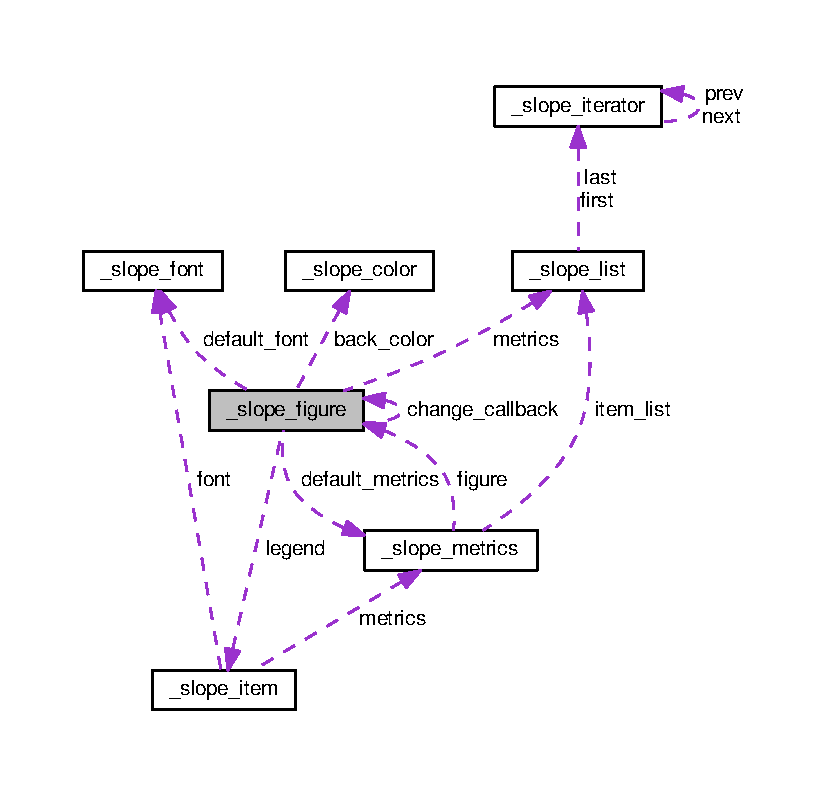
\includegraphics[width=350pt]{struct__slope__figure__coll__graph}
\end{center}
\end{figure}
\subsection*{Public Attributes}
\begin{DoxyCompactItemize}
\item 
\hypertarget{struct__slope__figure_a783cd1c9b86d7ddc6997a4b7e51b80df}{\hyperlink{group__List_ga88326d377deca937191acac6784bff0e}{slope\+\_\+list\+\_\+t} $\ast$ {\bfseries metrics}}\label{struct__slope__figure_a783cd1c9b86d7ddc6997a4b7e51b80df}

\item 
\hypertarget{struct__slope__figure_a76f248fab4d59b4170709525bca5883c}{\hyperlink{group__Metrics_gab80787ee8ae8dc449e770249fe0e3c35}{slope\+\_\+metrics\+\_\+t} $\ast$ {\bfseries default\+\_\+metrics}}\label{struct__slope__figure_a76f248fab4d59b4170709525bca5883c}

\item 
\hypertarget{struct__slope__figure_a1187fb125d8a66224dce9181887ed3c6}{\hyperlink{group__Primitives_ga29945f78eef5fcab497a3d15908b4b73}{slope\+\_\+font\+\_\+t} {\bfseries default\+\_\+font}}\label{struct__slope__figure_a1187fb125d8a66224dce9181887ed3c6}

\item 
\hypertarget{struct__slope__figure_ad5e0bd96cade55ef42f5a954322b0ac1}{\hyperlink{group__Item_ga2616141f0e164a876049da51ea3a8646}{slope\+\_\+item\+\_\+t} $\ast$ {\bfseries legend}}\label{struct__slope__figure_ad5e0bd96cade55ef42f5a954322b0ac1}

\item 
\hypertarget{struct__slope__figure_ab4d6de431e6f0b4a97b780b606ae0da3}{slope\+\_\+callback\+\_\+t {\bfseries change\+\_\+callback}}\label{struct__slope__figure_ab4d6de431e6f0b4a97b780b606ae0da3}

\item 
\hypertarget{struct__slope__figure_afce997af5c45b99ba7f123d40b5d0975}{\hyperlink{struct__slope__color}{slope\+\_\+color\+\_\+t} {\bfseries back\+\_\+color}}\label{struct__slope__figure_afce997af5c45b99ba7f123d40b5d0975}

\item 
\hypertarget{struct__slope__figure_ac29b1eb35fd245cf8603548bf360f415}{int {\bfseries fill\+\_\+back}}\label{struct__slope__figure_ac29b1eb35fd245cf8603548bf360f415}

\end{DoxyCompactItemize}


The documentation for this struct was generated from the following file\+:\begin{DoxyCompactItemize}
\item 
slope/figure\+\_\+p.\+h\end{DoxyCompactItemize}

\hypertarget{struct__slope__item}{\section{\+\_\+slope\+\_\+item Struct Reference}
\label{struct__slope__item}\index{\+\_\+slope\+\_\+item@{\+\_\+slope\+\_\+item}}
}


Collaboration diagram for \+\_\+slope\+\_\+item\+:
\subsection*{Public Attributes}
\begin{DoxyCompactItemize}
\item 
\hypertarget{struct__slope__item_add7193a54a1fabdb37cd26d048987395}{slope\+\_\+item\+\_\+class\+\_\+t $\ast$ {\bfseries klass}}\label{struct__slope__item_add7193a54a1fabdb37cd26d048987395}

\item 
\hypertarget{struct__slope__item_ac7bdb1cdc4aaf1fd8ae234eebc1e8e13}{\hyperlink{group__Metrics_gab80787ee8ae8dc449e770249fe0e3c35}{slope\+\_\+metrics\+\_\+t} $\ast$ {\bfseries metrics}}\label{struct__slope__item_ac7bdb1cdc4aaf1fd8ae234eebc1e8e13}

\item 
\hypertarget{struct__slope__item_a3a154a02eef112186595310fd7270769}{char $\ast$ {\bfseries name}}\label{struct__slope__item_a3a154a02eef112186595310fd7270769}

\item 
\hypertarget{struct__slope__item_ac8164345fdba3cc49b58dff578718f35}{int {\bfseries visible}}\label{struct__slope__item_ac8164345fdba3cc49b58dff578718f35}

\item 
\hypertarget{struct__slope__item_a3b8509ebb99801b1140a279aa79c629f}{int {\bfseries has\+\_\+thumb}}\label{struct__slope__item_a3b8509ebb99801b1140a279aa79c629f}

\end{DoxyCompactItemize}


The documentation for this struct was generated from the following file\+:\begin{DoxyCompactItemize}
\item 
slope/item\+\_\+p.\+h\end{DoxyCompactItemize}

\hypertarget{struct__slope__item__class}{\section{\+\_\+slope\+\_\+item\+\_\+class Struct Reference}
\label{struct__slope__item__class}\index{\+\_\+slope\+\_\+item\+\_\+class@{\+\_\+slope\+\_\+item\+\_\+class}}
}
\subsection*{Public Attributes}
\begin{DoxyCompactItemize}
\item 
\hypertarget{struct__slope__item__class_ae4ab90f79eb6bda572bea0477ca14462}{void($\ast$ {\bfseries destroy\+\_\+fn} )(\hyperlink{group__Item_ga2616141f0e164a876049da51ea3a8646}{slope\+\_\+item\+\_\+t} $\ast$)}\label{struct__slope__item__class_ae4ab90f79eb6bda572bea0477ca14462}

\item 
\hypertarget{struct__slope__item__class_ae5ab35bbf8653c59ad6fa0a37757cc9f}{void($\ast$ {\bfseries draw\+\_\+fn} )(\hyperlink{group__Item_ga2616141f0e164a876049da51ea3a8646}{slope\+\_\+item\+\_\+t} $\ast$, cairo\+\_\+t $\ast$, const \hyperlink{group__Metrics_gab80787ee8ae8dc449e770249fe0e3c35}{slope\+\_\+metrics\+\_\+t} $\ast$)}\label{struct__slope__item__class_ae5ab35bbf8653c59ad6fa0a37757cc9f}

\item 
\hypertarget{struct__slope__item__class_a290befa5d0305d18c40bdc3469ecd366}{void($\ast$ {\bfseries draw\+\_\+thumb\+\_\+fn} )(\hyperlink{group__Item_ga2616141f0e164a876049da51ea3a8646}{slope\+\_\+item\+\_\+t} $\ast$, const \hyperlink{struct__slope__point}{slope\+\_\+point\+\_\+t} $\ast$, cairo\+\_\+t $\ast$)}\label{struct__slope__item__class_a290befa5d0305d18c40bdc3469ecd366}

\end{DoxyCompactItemize}


The documentation for this struct was generated from the following file\+:\begin{DoxyCompactItemize}
\item 
slope/item\+\_\+p.\+h\end{DoxyCompactItemize}

\hypertarget{struct__slope__iterator}{\section{\+\_\+slope\+\_\+iterator Struct Reference}
\label{struct__slope__iterator}\index{\+\_\+slope\+\_\+iterator@{\+\_\+slope\+\_\+iterator}}
}


Collaboration diagram for \+\_\+slope\+\_\+iterator\+:
\nopagebreak
\begin{figure}[H]
\begin{center}
\leavevmode
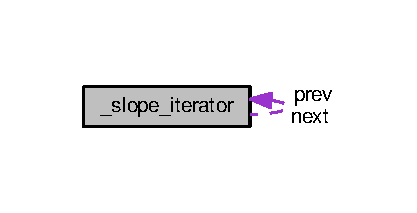
\includegraphics[width=200pt]{struct__slope__iterator__coll__graph}
\end{center}
\end{figure}
\subsection*{Public Attributes}
\begin{DoxyCompactItemize}
\item 
\hypertarget{struct__slope__iterator_a2e350fc606387696fa30b8bf28f65b81}{struct \hyperlink{struct__slope__iterator}{\+\_\+slope\+\_\+iterator} $\ast$ {\bfseries next}}\label{struct__slope__iterator_a2e350fc606387696fa30b8bf28f65b81}

\item 
\hypertarget{struct__slope__iterator_ad1f3246238c01985972820139a2729dd}{struct \hyperlink{struct__slope__iterator}{\+\_\+slope\+\_\+iterator} $\ast$ {\bfseries prev}}\label{struct__slope__iterator_ad1f3246238c01985972820139a2729dd}

\item 
\hypertarget{struct__slope__iterator_af9a1a22abb8ffc7b7a67cdf58be7aa6f}{void $\ast$ {\bfseries data}}\label{struct__slope__iterator_af9a1a22abb8ffc7b7a67cdf58be7aa6f}

\end{DoxyCompactItemize}


The documentation for this struct was generated from the following file\+:\begin{DoxyCompactItemize}
\item 
slope/list.\+c\end{DoxyCompactItemize}

\hypertarget{struct__slope__legend}{\section{\+\_\+slope\+\_\+legend Struct Reference}
\label{struct__slope__legend}\index{\+\_\+slope\+\_\+legend@{\+\_\+slope\+\_\+legend}}
}


Collaboration diagram for \+\_\+slope\+\_\+legend\+:
\subsection*{Public Attributes}
\begin{DoxyCompactItemize}
\item 
\hypertarget{struct__slope__legend_aced1e1584bd8ba4cbe7ffc3ad0dadc44}{\hyperlink{group__Item_ga2616141f0e164a876049da51ea3a8646}{slope\+\_\+item\+\_\+t} {\bfseries parent}}\label{struct__slope__legend_aced1e1584bd8ba4cbe7ffc3ad0dadc44}

\item 
\hypertarget{struct__slope__legend_ae18a7deffb619252b055672110703bb9}{\hyperlink{struct__slope__rect}{slope\+\_\+rect\+\_\+t} {\bfseries rect}}\label{struct__slope__legend_ae18a7deffb619252b055672110703bb9}

\item 
\hypertarget{struct__slope__legend_a1abf347ffdf1ce3630e03ef93bc79a3b}{\hyperlink{struct__slope__color}{slope\+\_\+color\+\_\+t} {\bfseries fill\+\_\+color}}\label{struct__slope__legend_a1abf347ffdf1ce3630e03ef93bc79a3b}

\item 
\hypertarget{struct__slope__legend_a9be59a3fcd403e9455211399c9dabe9e}{\hyperlink{struct__slope__color}{slope\+\_\+color\+\_\+t} {\bfseries stroke\+\_\+color}}\label{struct__slope__legend_a9be59a3fcd403e9455211399c9dabe9e}

\item 
\hypertarget{struct__slope__legend_aac6517fed40bc604f90d188c88c39c8b}{slope\+\_\+legend\+\_\+position\+\_\+t {\bfseries position}}\label{struct__slope__legend_aac6517fed40bc604f90d188c88c39c8b}

\end{DoxyCompactItemize}


The documentation for this struct was generated from the following file\+:\begin{DoxyCompactItemize}
\item 
slope/legend\+\_\+p.\+h\end{DoxyCompactItemize}

\hypertarget{struct__slope__list}{\section{\+\_\+slope\+\_\+list Struct Reference}
\label{struct__slope__list}\index{\+\_\+slope\+\_\+list@{\+\_\+slope\+\_\+list}}
}


Collaboration diagram for \+\_\+slope\+\_\+list\+:
\subsection*{Public Attributes}
\begin{DoxyCompactItemize}
\item 
\hypertarget{struct__slope__list_ae4755b2ce5e8e2894fd42f99a803b6ee}{struct \hyperlink{struct__slope__iterator}{\+\_\+slope\+\_\+iterator} $\ast$ {\bfseries first}}\label{struct__slope__list_ae4755b2ce5e8e2894fd42f99a803b6ee}

\item 
\hypertarget{struct__slope__list_a83a3ca98c4f39466fec5a1caf37c975b}{struct \hyperlink{struct__slope__iterator}{\+\_\+slope\+\_\+iterator} $\ast$ {\bfseries last}}\label{struct__slope__list_a83a3ca98c4f39466fec5a1caf37c975b}

\item 
\hypertarget{struct__slope__list_a36ba8b99c1187709b8c489815bea4413}{int {\bfseries size}}\label{struct__slope__list_a36ba8b99c1187709b8c489815bea4413}

\end{DoxyCompactItemize}


The documentation for this struct was generated from the following file\+:\begin{DoxyCompactItemize}
\item 
slope/list.\+c\end{DoxyCompactItemize}

\hypertarget{struct__slope__metrics}{\section{\+\_\+slope\+\_\+metrics Struct Reference}
\label{struct__slope__metrics}\index{\+\_\+slope\+\_\+metrics@{\+\_\+slope\+\_\+metrics}}
}


Collaboration diagram for \+\_\+slope\+\_\+metrics\+:
\subsection*{Public Attributes}
\begin{DoxyCompactItemize}
\item 
\hypertarget{struct__slope__metrics_ac0be13f740c34881ef12ee711d02c4ab}{slope\+\_\+metrics\+\_\+class\+\_\+t $\ast$ {\bfseries klass}}\label{struct__slope__metrics_ac0be13f740c34881ef12ee711d02c4ab}

\item 
\hypertarget{struct__slope__metrics_a3aa8ff6d674059c26e68980d6196d655}{slope\+\_\+metrics\+\_\+type\+\_\+t {\bfseries type}}\label{struct__slope__metrics_a3aa8ff6d674059c26e68980d6196d655}

\item 
\hypertarget{struct__slope__metrics_a90f058e9225cd913f585c36739f95901}{\hyperlink{group__Figure_ga507cc82eeca8255d6c0f603ffdaeb59e}{slope\+\_\+figure\+\_\+t} $\ast$ {\bfseries figure}}\label{struct__slope__metrics_a90f058e9225cd913f585c36739f95901}

\item 
\hypertarget{struct__slope__metrics_a0a920646d930ff607bb8fc954b1cafbc}{\hyperlink{struct__slope__list}{slope\+\_\+list\+\_\+t} $\ast$ {\bfseries item\+\_\+list}}\label{struct__slope__metrics_a0a920646d930ff607bb8fc954b1cafbc}

\item 
\hypertarget{struct__slope__metrics_aa91b6061f72089b60903d8310d691464}{double {\bfseries x\+\_\+low\+\_\+bound}}\label{struct__slope__metrics_aa91b6061f72089b60903d8310d691464}

\item 
\hypertarget{struct__slope__metrics_a04c15859cae09965d4608144f87016c2}{double {\bfseries x\+\_\+up\+\_\+bound}}\label{struct__slope__metrics_a04c15859cae09965d4608144f87016c2}

\item 
\hypertarget{struct__slope__metrics_acdba84cfba06e6293e18ba29cc822e35}{double {\bfseries y\+\_\+low\+\_\+bound}}\label{struct__slope__metrics_acdba84cfba06e6293e18ba29cc822e35}

\item 
\hypertarget{struct__slope__metrics_a7586b1c1f9cd7f80e929d3818534a20c}{double {\bfseries y\+\_\+up\+\_\+bound}}\label{struct__slope__metrics_a7586b1c1f9cd7f80e929d3818534a20c}

\item 
\hypertarget{struct__slope__metrics_a435925cdf5bd35658acfb48dcd707b66}{double {\bfseries xmin\+\_\+figure}}\label{struct__slope__metrics_a435925cdf5bd35658acfb48dcd707b66}

\item 
\hypertarget{struct__slope__metrics_ae5a8b9e2c17313f5e8df3ba3a3d29fd2}{double {\bfseries xmax\+\_\+figure}}\label{struct__slope__metrics_ae5a8b9e2c17313f5e8df3ba3a3d29fd2}

\item 
\hypertarget{struct__slope__metrics_a6000828f5bc6d9c83d66aa7899ff36dc}{double {\bfseries ymin\+\_\+figure}}\label{struct__slope__metrics_a6000828f5bc6d9c83d66aa7899ff36dc}

\item 
\hypertarget{struct__slope__metrics_a7351a93e448f8dd9441d9319fd984ac7}{double {\bfseries ymax\+\_\+figure}}\label{struct__slope__metrics_a7351a93e448f8dd9441d9319fd984ac7}

\item 
\hypertarget{struct__slope__metrics_a6c276a074789c36f794b053afc0e7267}{double {\bfseries width\+\_\+figure}}\label{struct__slope__metrics_a6c276a074789c36f794b053afc0e7267}

\item 
\hypertarget{struct__slope__metrics_a2251d1d4ddf5113421470ee169821d0b}{double {\bfseries height\+\_\+figure}}\label{struct__slope__metrics_a2251d1d4ddf5113421470ee169821d0b}

\item 
\hypertarget{struct__slope__metrics_a33d100a34f52fce1834dcb7766466fd0}{int {\bfseries visible}}\label{struct__slope__metrics_a33d100a34f52fce1834dcb7766466fd0}

\end{DoxyCompactItemize}


The documentation for this struct was generated from the following file\+:\begin{DoxyCompactItemize}
\item 
slope/metrics\+\_\+p.\+h\end{DoxyCompactItemize}

\hypertarget{struct__slope__metrics__class}{\section{\+\_\+slope\+\_\+metrics\+\_\+class Struct Reference}
\label{struct__slope__metrics__class}\index{\+\_\+slope\+\_\+metrics\+\_\+class@{\+\_\+slope\+\_\+metrics\+\_\+class}}
}
\subsection*{Public Attributes}
\begin{DoxyCompactItemize}
\item 
\hypertarget{struct__slope__metrics__class_a4368bec8121a13cd6f65bfd004237345}{void($\ast$ {\bfseries destroy\+\_\+fn} )(\hyperlink{group__Metrics_gab80787ee8ae8dc449e770249fe0e3c35}{slope\+\_\+metrics\+\_\+t} $\ast$)}\label{struct__slope__metrics__class_a4368bec8121a13cd6f65bfd004237345}

\item 
\hypertarget{struct__slope__metrics__class_afdb9e43174fa9f4cacfa7dce2b5e8368}{void($\ast$ {\bfseries update\+\_\+fn} )(\hyperlink{group__Metrics_gab80787ee8ae8dc449e770249fe0e3c35}{slope\+\_\+metrics\+\_\+t} $\ast$)}\label{struct__slope__metrics__class_afdb9e43174fa9f4cacfa7dce2b5e8368}

\item 
\hypertarget{struct__slope__metrics__class_adc93586637602cdb8805965d29de2ab0}{void($\ast$ {\bfseries draw\+\_\+fn} )(\hyperlink{group__Metrics_gab80787ee8ae8dc449e770249fe0e3c35}{slope\+\_\+metrics\+\_\+t} $\ast$, cairo\+\_\+t $\ast$, const \hyperlink{struct__slope__rect}{slope\+\_\+rect\+\_\+t} $\ast$)}\label{struct__slope__metrics__class_adc93586637602cdb8805965d29de2ab0}

\end{DoxyCompactItemize}


The documentation for this struct was generated from the following file\+:\begin{DoxyCompactItemize}
\item 
slope/metrics\+\_\+p.\+h\end{DoxyCompactItemize}

\hypertarget{struct__slope__point}{\section{\+\_\+slope\+\_\+point Struct Reference}
\label{struct__slope__point}\index{\+\_\+slope\+\_\+point@{\+\_\+slope\+\_\+point}}
}
\subsection*{Public Attributes}
\begin{DoxyCompactItemize}
\item 
\hypertarget{struct__slope__point_a75e2ad1b976a451b7eabebce220a9718}{double {\bfseries x}}\label{struct__slope__point_a75e2ad1b976a451b7eabebce220a9718}

\item 
\hypertarget{struct__slope__point_a2dc7b075530ba3e2a8add8c0e03ace8c}{double {\bfseries y}}\label{struct__slope__point_a2dc7b075530ba3e2a8add8c0e03ace8c}

\end{DoxyCompactItemize}


The documentation for this struct was generated from the following file\+:\begin{DoxyCompactItemize}
\item 
slope/\hyperlink{primitives_8h}{primitives.\+h}\end{DoxyCompactItemize}

\hypertarget{struct__slope__rect}{\section{\+\_\+slope\+\_\+rect Struct Reference}
\label{struct__slope__rect}\index{\+\_\+slope\+\_\+rect@{\+\_\+slope\+\_\+rect}}
}
\subsection*{Public Attributes}
\begin{DoxyCompactItemize}
\item 
\hypertarget{struct__slope__rect_a50861a894de903db2ee81e7d47d35e47}{double {\bfseries x}}\label{struct__slope__rect_a50861a894de903db2ee81e7d47d35e47}

\item 
\hypertarget{struct__slope__rect_a6973dc88937c8034771edfc69288feb0}{double {\bfseries y}}\label{struct__slope__rect_a6973dc88937c8034771edfc69288feb0}

\item 
\hypertarget{struct__slope__rect_a09583ea10ed82dd3fe64da7e7a6bfb24}{double {\bfseries width}}\label{struct__slope__rect_a09583ea10ed82dd3fe64da7e7a6bfb24}

\item 
\hypertarget{struct__slope__rect_aee8ea863cafdbee525219b26bd400177}{double {\bfseries height}}\label{struct__slope__rect_aee8ea863cafdbee525219b26bd400177}

\end{DoxyCompactItemize}


The documentation for this struct was generated from the following file\+:\begin{DoxyCompactItemize}
\item 
slope/\hyperlink{primitives_8h}{primitives.\+h}\end{DoxyCompactItemize}

\hypertarget{struct__slope__vector}{\section{\+\_\+slope\+\_\+vector Struct Reference}
\label{struct__slope__vector}\index{\+\_\+slope\+\_\+vector@{\+\_\+slope\+\_\+vector}}
}
\subsection*{Public Attributes}
\begin{DoxyCompactItemize}
\item 
\hypertarget{struct__slope__vector_a7b6b1ef243e1c3a288ec1ae932512e1f}{double $\ast$ {\bfseries v}}\label{struct__slope__vector_a7b6b1ef243e1c3a288ec1ae932512e1f}

\item 
\hypertarget{struct__slope__vector_a2bea13c3c5345b2540bf810ef117e7ab}{int {\bfseries nalloc}}\label{struct__slope__vector_a2bea13c3c5345b2540bf810ef117e7ab}

\item 
\hypertarget{struct__slope__vector_a2635b20c85067423e4f3482e9557613e}{int {\bfseries size}}\label{struct__slope__vector_a2635b20c85067423e4f3482e9557613e}

\end{DoxyCompactItemize}


The documentation for this struct was generated from the following file\+:\begin{DoxyCompactItemize}
\item 
slope/vector.\+h\end{DoxyCompactItemize}

\hypertarget{struct__slope__xyaxis}{\section{\+\_\+slope\+\_\+xyaxis Struct Reference}
\label{struct__slope__xyaxis}\index{\+\_\+slope\+\_\+xyaxis@{\+\_\+slope\+\_\+xyaxis}}
}


Collaboration diagram for \+\_\+slope\+\_\+xyaxis\+:
\subsection*{Public Attributes}
\begin{DoxyCompactItemize}
\item 
\hypertarget{struct__slope__xyaxis_ab53d8e2917569ff2ba7d4df2fdf89d05}{\hyperlink{group__Item_ga2616141f0e164a876049da51ea3a8646}{slope\+\_\+item\+\_\+t} {\bfseries parent}}\label{struct__slope__xyaxis_ab53d8e2917569ff2ba7d4df2fdf89d05}

\item 
\hypertarget{struct__slope__xyaxis_a56aa7533e274304b0391a18a5c1e760c}{slope\+\_\+xyaxis\+\_\+type\+\_\+t {\bfseries type}}\label{struct__slope__xyaxis_a56aa7533e274304b0391a18a5c1e760c}

\item 
\hypertarget{struct__slope__xyaxis_afbee67325cf0615e6897aa608660024f}{\hyperlink{struct__slope__color}{slope\+\_\+color\+\_\+t} {\bfseries color}}\label{struct__slope__xyaxis_afbee67325cf0615e6897aa608660024f}

\item 
\hypertarget{struct__slope__xyaxis_a6a1eecc666de23bfd52da363a8452ac5}{double {\bfseries length}}\label{struct__slope__xyaxis_a6a1eecc666de23bfd52da363a8452ac5}

\item 
\hypertarget{struct__slope__xyaxis_a815c7ca4b34489e3f85cfb3b0272bd55}{double {\bfseries divlen}}\label{struct__slope__xyaxis_a815c7ca4b34489e3f85cfb3b0272bd55}

\item 
\hypertarget{struct__slope__xyaxis_addc6da873f46da73c1233d2343ed92b9}{int {\bfseries divnum}}\label{struct__slope__xyaxis_addc6da873f46da73c1233d2343ed92b9}

\end{DoxyCompactItemize}


The documentation for this struct was generated from the following file\+:\begin{DoxyCompactItemize}
\item 
slope/xyaxis\+\_\+p.\+h\end{DoxyCompactItemize}

\hypertarget{struct__slope__xyitem}{\section{\+\_\+slope\+\_\+xyitem Struct Reference}
\label{struct__slope__xyitem}\index{\+\_\+slope\+\_\+xyitem@{\+\_\+slope\+\_\+xyitem}}
}


Collaboration diagram for \+\_\+slope\+\_\+xyitem\+:
\nopagebreak
\begin{figure}[H]
\begin{center}
\leavevmode
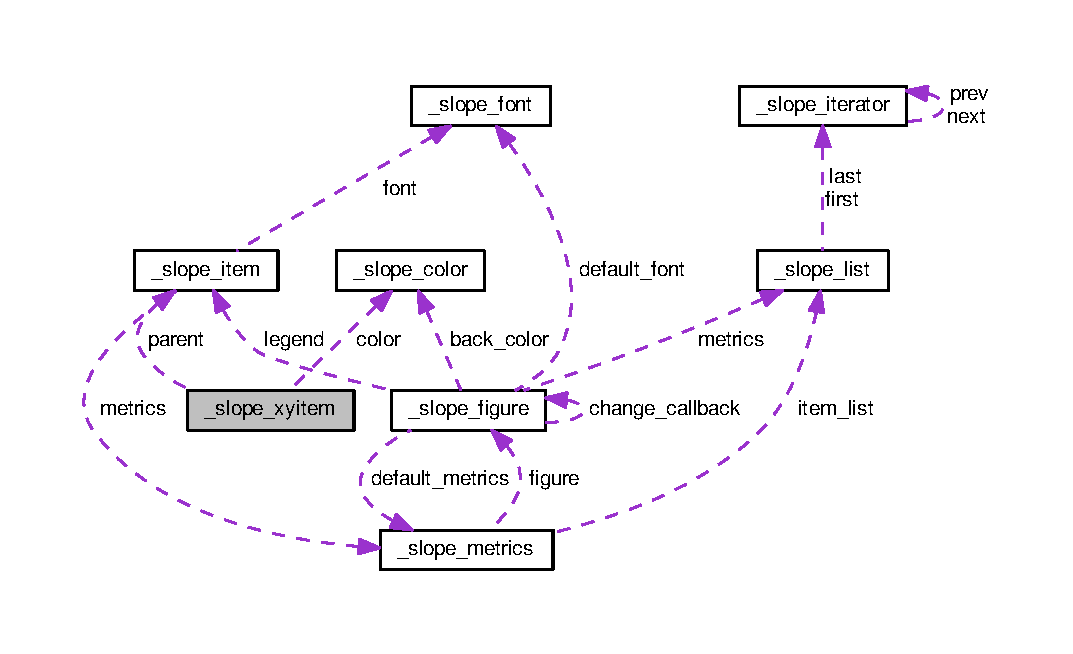
\includegraphics[width=350pt]{struct__slope__xyitem__coll__graph}
\end{center}
\end{figure}
\subsection*{Public Attributes}
\begin{DoxyCompactItemize}
\item 
\hypertarget{struct__slope__xyitem_a84f281e8c4ec73ed02f8b85e594319b6}{\hyperlink{group__Item_ga2616141f0e164a876049da51ea3a8646}{slope\+\_\+item\+\_\+t} {\bfseries parent}}\label{struct__slope__xyitem_a84f281e8c4ec73ed02f8b85e594319b6}

\item 
\hypertarget{struct__slope__xyitem_a5b9268cd9e371fcd22002ebed979bb8a}{int {\bfseries rescalable}}\label{struct__slope__xyitem_a5b9268cd9e371fcd22002ebed979bb8a}

\item 
\hypertarget{struct__slope__xyitem_ae1493e872601ce918c5874e187a55a3c}{const double $\ast$ {\bfseries vx}}\label{struct__slope__xyitem_ae1493e872601ce918c5874e187a55a3c}

\item 
\hypertarget{struct__slope__xyitem_a133d040cfe16cf85e26568e5213cb950}{const double $\ast$ {\bfseries vy}}\label{struct__slope__xyitem_a133d040cfe16cf85e26568e5213cb950}

\item 
\hypertarget{struct__slope__xyitem_a77d380f8d9d0700bb2349d256e36a2b4}{int {\bfseries n}}\label{struct__slope__xyitem_a77d380f8d9d0700bb2349d256e36a2b4}

\item 
\hypertarget{struct__slope__xyitem_a7d2cb6e80d6d6ce215e871a72349e570}{double {\bfseries xmin}}\label{struct__slope__xyitem_a7d2cb6e80d6d6ce215e871a72349e570}

\item 
\hypertarget{struct__slope__xyitem_a920a8c4003cf2648a92b38cae4a2230b}{double {\bfseries xmax}}\label{struct__slope__xyitem_a920a8c4003cf2648a92b38cae4a2230b}

\item 
\hypertarget{struct__slope__xyitem_a2fde7ba32d219624978c2b5efbb0ae24}{double {\bfseries ymin}}\label{struct__slope__xyitem_a2fde7ba32d219624978c2b5efbb0ae24}

\item 
\hypertarget{struct__slope__xyitem_a59b258bcde73db7e1246b2258fcb4cf4}{double {\bfseries ymax}}\label{struct__slope__xyitem_a59b258bcde73db7e1246b2258fcb4cf4}

\item 
\hypertarget{struct__slope__xyitem_a15d5849f6c2fea2fac75d483eabe198a}{\hyperlink{struct__slope__color}{slope\+\_\+color\+\_\+t} {\bfseries color}}\label{struct__slope__xyitem_a15d5849f6c2fea2fac75d483eabe198a}

\item 
\hypertarget{struct__slope__xyitem_afbec1ee0523a97e576b2a369d909c888}{\hyperlink{group__Item_ga7be66725a3a198bcbd9434e6d3ad70c5}{slope\+\_\+scatter\+\_\+t} {\bfseries scatter}}\label{struct__slope__xyitem_afbec1ee0523a97e576b2a369d909c888}

\item 
\hypertarget{struct__slope__xyitem_aa4f942a3bc1907d54158df9912cbfed6}{int {\bfseries fill\+\_\+symbol}}\label{struct__slope__xyitem_aa4f942a3bc1907d54158df9912cbfed6}

\item 
\hypertarget{struct__slope__xyitem_a809b4363b4fae543e0196983bcc99bd4}{int {\bfseries antialias}}\label{struct__slope__xyitem_a809b4363b4fae543e0196983bcc99bd4}

\item 
\hypertarget{struct__slope__xyitem_afa9758ee875e6c37ed250eb0d6cc4d4b}{double {\bfseries line\+\_\+width}}\label{struct__slope__xyitem_afa9758ee875e6c37ed250eb0d6cc4d4b}

\end{DoxyCompactItemize}


The documentation for this struct was generated from the following file\+:\begin{DoxyCompactItemize}
\item 
slope/xyitem\+\_\+p.\+h\end{DoxyCompactItemize}

\hypertarget{struct__slope__xymetrics}{\section{\+\_\+slope\+\_\+xymetrics Struct Reference}
\label{struct__slope__xymetrics}\index{\+\_\+slope\+\_\+xymetrics@{\+\_\+slope\+\_\+xymetrics}}
}


Collaboration diagram for \+\_\+slope\+\_\+xymetrics\+:
\subsection*{Public Attributes}
\begin{DoxyCompactItemize}
\item 
\hypertarget{struct__slope__xymetrics_aec0f7546c89f84b770fe7967602f8b5f}{\hyperlink{group__Metrics_gab80787ee8ae8dc449e770249fe0e3c35}{slope\+\_\+metrics\+\_\+t} {\bfseries parent}}\label{struct__slope__xymetrics_aec0f7546c89f84b770fe7967602f8b5f}

\item 
\hypertarget{struct__slope__xymetrics_a0872d22ecbf7129241bf947cfef15769}{\hyperlink{struct__slope__list}{slope\+\_\+list\+\_\+t} $\ast$ {\bfseries axis\+\_\+list}}\label{struct__slope__xymetrics_a0872d22ecbf7129241bf947cfef15769}

\item 
\hypertarget{struct__slope__xymetrics_ad1d3347be073c3d5e54dcc4fcf8be3f0}{double {\bfseries xmin}}\label{struct__slope__xymetrics_ad1d3347be073c3d5e54dcc4fcf8be3f0}

\item 
\hypertarget{struct__slope__xymetrics_a1b5bc871445b58a36fdbd8fda316da64}{double {\bfseries xmax}}\label{struct__slope__xymetrics_a1b5bc871445b58a36fdbd8fda316da64}

\item 
\hypertarget{struct__slope__xymetrics_a0185807d2c62875950fb1001005ee0b3}{double {\bfseries ymin}}\label{struct__slope__xymetrics_a0185807d2c62875950fb1001005ee0b3}

\item 
\hypertarget{struct__slope__xymetrics_a68d0668dd3b423c8fb44fe943cfaaed6}{double {\bfseries ymax}}\label{struct__slope__xymetrics_a68d0668dd3b423c8fb44fe943cfaaed6}

\item 
\hypertarget{struct__slope__xymetrics_adecdb95c1bc9394ea4332c2182539153}{double {\bfseries width}}\label{struct__slope__xymetrics_adecdb95c1bc9394ea4332c2182539153}

\item 
\hypertarget{struct__slope__xymetrics_a51349b89d2fb960fe1503ac3104d80d0}{double {\bfseries height}}\label{struct__slope__xymetrics_a51349b89d2fb960fe1503ac3104d80d0}

\end{DoxyCompactItemize}


The documentation for this struct was generated from the following file\+:\begin{DoxyCompactItemize}
\item 
slope/xymetrics\+\_\+p.\+h\end{DoxyCompactItemize}

\hypertarget{struct__SlopeView}{\section{\+\_\+\+Slope\+View Struct Reference}
\label{struct__SlopeView}\index{\+\_\+\+Slope\+View@{\+\_\+\+Slope\+View}}
}
\subsection*{Public Attributes}
\begin{DoxyCompactItemize}
\item 
\hypertarget{struct__SlopeView_ae74ce5afc47d1f5d2aa1bb45f822377c}{Gtk\+Drawing\+Area {\bfseries parent}}\label{struct__SlopeView_ae74ce5afc47d1f5d2aa1bb45f822377c}

\end{DoxyCompactItemize}


The documentation for this struct was generated from the following file\+:\begin{DoxyCompactItemize}
\item 
slope/view.\+h\end{DoxyCompactItemize}

\hypertarget{struct__SlopeViewClass}{\section{\+\_\+\+Slope\+View\+Class Struct Reference}
\label{struct__SlopeViewClass}\index{\+\_\+\+Slope\+View\+Class@{\+\_\+\+Slope\+View\+Class}}
}
\subsection*{Public Attributes}
\begin{DoxyCompactItemize}
\item 
\hypertarget{struct__SlopeViewClass_a169832130ff08b762fd07bc5021c9f56}{Gtk\+Drawing\+Area\+Class {\bfseries parent}}\label{struct__SlopeViewClass_a169832130ff08b762fd07bc5021c9f56}

\end{DoxyCompactItemize}


The documentation for this struct was generated from the following file\+:\begin{DoxyCompactItemize}
\item 
slope/view.\+h\end{DoxyCompactItemize}

\hypertarget{struct__SlopeViewPrivate}{\section{\+\_\+\+Slope\+View\+Private Struct Reference}
\label{struct__SlopeViewPrivate}\index{\+\_\+\+Slope\+View\+Private@{\+\_\+\+Slope\+View\+Private}}
}


Collaboration diagram for \+\_\+\+Slope\+View\+Private\+:
\nopagebreak
\begin{figure}[H]
\begin{center}
\leavevmode
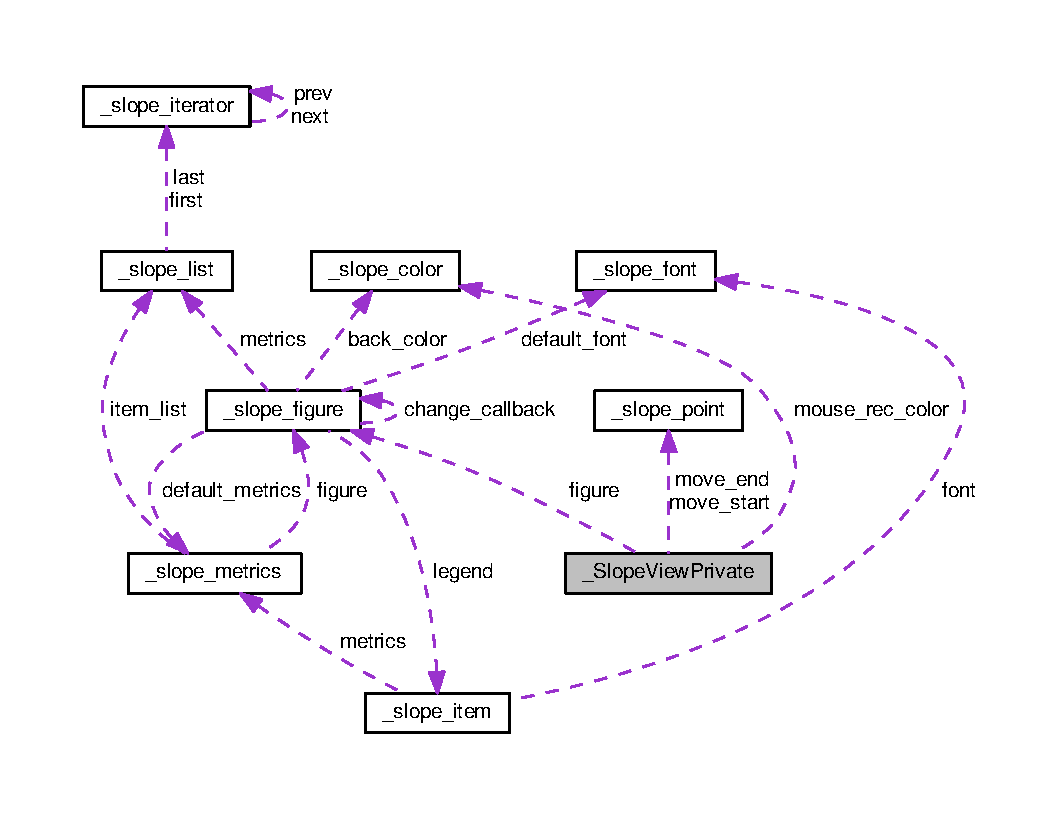
\includegraphics[width=350pt]{struct__SlopeViewPrivate__coll__graph}
\end{center}
\end{figure}
\subsection*{Public Attributes}
\begin{DoxyCompactItemize}
\item 
\hypertarget{struct__SlopeViewPrivate_aafdec47c695b1fb1ed2374f55d4345ae}{\hyperlink{group__Figure_ga507cc82eeca8255d6c0f603ffdaeb59e}{slope\+\_\+figure\+\_\+t} $\ast$ {\bfseries figure}}\label{struct__SlopeViewPrivate_aafdec47c695b1fb1ed2374f55d4345ae}

\item 
\hypertarget{struct__SlopeViewPrivate_aa85fbecab3e04e09e70268e513a51aad}{cairo\+\_\+surface\+\_\+t $\ast$ {\bfseries back\+\_\+surf}}\label{struct__SlopeViewPrivate_aa85fbecab3e04e09e70268e513a51aad}

\item 
\hypertarget{struct__SlopeViewPrivate_a19d3d175ce68cbf2e30cd85249e7edf6}{\hyperlink{struct__slope__point}{slope\+\_\+point\+\_\+t} {\bfseries move\+\_\+start}}\label{struct__SlopeViewPrivate_a19d3d175ce68cbf2e30cd85249e7edf6}

\item 
\hypertarget{struct__SlopeViewPrivate_a1ff87d94e9ce2bfe356f4263e67a32cd}{\hyperlink{struct__slope__point}{slope\+\_\+point\+\_\+t} {\bfseries move\+\_\+end}}\label{struct__SlopeViewPrivate_a1ff87d94e9ce2bfe356f4263e67a32cd}

\item 
\hypertarget{struct__SlopeViewPrivate_ab248d01239b98c865d508e41aa38ac1e}{\hyperlink{struct__slope__color}{slope\+\_\+color\+\_\+t} {\bfseries mouse\+\_\+rec\+\_\+color}}\label{struct__SlopeViewPrivate_ab248d01239b98c865d508e41aa38ac1e}

\item 
\hypertarget{struct__SlopeViewPrivate_afb48401b5966a0e545d0062797143176}{\hyperlink{group__Primitives_gac55afa016ca777119a6c343d1655d558}{slope\+\_\+bool\+\_\+t} {\bfseries mouse\+\_\+zoom}}\label{struct__SlopeViewPrivate_afb48401b5966a0e545d0062797143176}

\item 
\hypertarget{struct__SlopeViewPrivate_a956462aa9254d2beff0581b7449017c9}{int {\bfseries on\+\_\+move}}\label{struct__SlopeViewPrivate_a956462aa9254d2beff0581b7449017c9}

\item 
\hypertarget{struct__SlopeViewPrivate_a87e2e6ba1fa27e792bd82b8fb1658615}{int {\bfseries press\+\_\+sig\+\_\+id}}\label{struct__SlopeViewPrivate_a87e2e6ba1fa27e792bd82b8fb1658615}

\item 
\hypertarget{struct__SlopeViewPrivate_a027e97def0a6bde19c2e9ec2daa7a754}{int {\bfseries move\+\_\+sig\+\_\+id}}\label{struct__SlopeViewPrivate_a027e97def0a6bde19c2e9ec2daa7a754}

\item 
\hypertarget{struct__SlopeViewPrivate_a1c2d5d2faac3c86ad07877c415127580}{int {\bfseries release\+\_\+sig\+\_\+id}}\label{struct__SlopeViewPrivate_a1c2d5d2faac3c86ad07877c415127580}

\end{DoxyCompactItemize}


The documentation for this struct was generated from the following file\+:\begin{DoxyCompactItemize}
\item 
slope/view.\+c\end{DoxyCompactItemize}

\chapter{File Documentation}
\hypertarget{figure_8h}{\section{slope/figure.h File Reference}
\label{figure_8h}\index{slope/figure.\+h@{slope/figure.\+h}}
}
{\ttfamily \#include \char`\"{}slope/list.\+h\char`\"{}}\\*
{\ttfamily \#include \char`\"{}slope/primitives.\+h\char`\"{}}\\*
Include dependency graph for figure.\+h\+:
This graph shows which files directly or indirectly include this file\+:
\subsection*{Functions}
\begin{DoxyCompactItemize}
\item 
S\+L\+O\+P\+E\+\_\+\+B\+E\+G\+I\+N\+\_\+\+D\+E\+C\+L\+S slope\+\_\+public \\*
\hyperlink{group__Figure_ga507cc82eeca8255d6c0f603ffdaeb59e}{slope\+\_\+figure\+\_\+t} $\ast$ \hyperlink{group__Figure_ga0534b5fef88fda65fd4b8feb33071cab}{slope\+\_\+figure\+\_\+create} ()
\begin{DoxyCompactList}\small\item\em Creates a new figure object. \end{DoxyCompactList}\item 
slope\+\_\+public \hyperlink{group__List_ga88326d377deca937191acac6784bff0e}{slope\+\_\+list\+\_\+t} $\ast$ \hyperlink{group__Figure_gac7d6aaca4df6806f00f3cb130a78dcde}{slope\+\_\+figure\+\_\+get\+\_\+metrics\+\_\+list} (const \hyperlink{group__Figure_ga507cc82eeca8255d6c0f603ffdaeb59e}{slope\+\_\+figure\+\_\+t} $\ast$figure)
\begin{DoxyCompactList}\small\item\em Retrieves the metrics list of figure. \end{DoxyCompactList}\item 
\hypertarget{group__Figure_ga08b6896169ef4a926e7d487ade3fe74e}{slope\+\_\+public void \hyperlink{group__Figure_ga08b6896169ef4a926e7d487ade3fe74e}{slope\+\_\+figure\+\_\+add\+\_\+metrics} (\hyperlink{group__Figure_ga507cc82eeca8255d6c0f603ffdaeb59e}{slope\+\_\+figure\+\_\+t} $\ast$figure, \hyperlink{group__Metrics_gab80787ee8ae8dc449e770249fe0e3c35}{slope\+\_\+metrics\+\_\+t} $\ast$metrics)}\label{group__Figure_ga08b6896169ef4a926e7d487ade3fe74e}

\begin{DoxyCompactList}\small\item\em Adds a metrics the metrics list of figure. \end{DoxyCompactList}\item 
\hypertarget{group__Figure_gada369b301fabc0c40ef172e22d4fcb85}{slope\+\_\+public void \hyperlink{group__Figure_gada369b301fabc0c40ef172e22d4fcb85}{slope\+\_\+figure\+\_\+destroy} (\hyperlink{group__Figure_ga507cc82eeca8255d6c0f603ffdaeb59e}{slope\+\_\+figure\+\_\+t} $\ast$figure)}\label{group__Figure_gada369b301fabc0c40ef172e22d4fcb85}

\begin{DoxyCompactList}\small\item\em Destroys any figure object and frees the memory used by it. \end{DoxyCompactList}\item 
slope\+\_\+public void \hyperlink{group__Figure_ga386e261642ba2b0fdc39a550e3e94462}{slope\+\_\+figure\+\_\+draw} (\hyperlink{group__Figure_ga507cc82eeca8255d6c0f603ffdaeb59e}{slope\+\_\+figure\+\_\+t} $\ast$figure, cairo\+\_\+t $\ast$cr, const \hyperlink{struct__slope__rect}{slope\+\_\+rect\+\_\+t} $\ast$rect)
\begin{DoxyCompactList}\small\item\em Draw the contents of this figure to one of cairo's backends via cr. \end{DoxyCompactList}\item 
slope\+\_\+public void \hyperlink{group__Figure_ga586a40d60b3c5feec3f74f1bb00b011d}{slope\+\_\+figure\+\_\+write\+\_\+to\+\_\+png} (\hyperlink{group__Figure_ga507cc82eeca8255d6c0f603ffdaeb59e}{slope\+\_\+figure\+\_\+t} $\ast$figure, const char $\ast$filename, int width, int height)
\begin{DoxyCompactList}\small\item\em Writes the figure to a png file. \end{DoxyCompactList}\item 
slope\+\_\+public int \hyperlink{group__Figure_ga18b13f5d94a871984760eaa4b5f5f4ae}{slope\+\_\+figure\+\_\+write\+\_\+to\+\_\+svg} (\hyperlink{group__Figure_ga507cc82eeca8255d6c0f603ffdaeb59e}{slope\+\_\+figure\+\_\+t} $\ast$figure, const char $\ast$filename, int width, int height)
\begin{DoxyCompactList}\small\item\em The figure to be drawn. \end{DoxyCompactList}\item 
slope\+\_\+public int \hyperlink{group__Figure_ga3d70896b8765c2ea7058e5213daa17fd}{slope\+\_\+figure\+\_\+write\+\_\+to\+\_\+pdf} (\hyperlink{group__Figure_ga507cc82eeca8255d6c0f603ffdaeb59e}{slope\+\_\+figure\+\_\+t} $\ast$figure, const char $\ast$filename, int width, int height)
\begin{DoxyCompactList}\small\item\em The figure to be drawn. \end{DoxyCompactList}\item 
slope\+\_\+public int \hyperlink{group__Figure_gaad033abcd87cdbae258f073c6f43101b}{slope\+\_\+figure\+\_\+write\+\_\+to\+\_\+ps} (\hyperlink{group__Figure_ga507cc82eeca8255d6c0f603ffdaeb59e}{slope\+\_\+figure\+\_\+t} $\ast$figure, const char $\ast$filename, int width, int height)
\begin{DoxyCompactList}\small\item\em The figure to be drawn. \end{DoxyCompactList}\item 
slope\+\_\+public \hyperlink{group__Metrics_gab80787ee8ae8dc449e770249fe0e3c35}{slope\+\_\+metrics\+\_\+t} $\ast$ \hyperlink{group__Figure_gae97736e589280dfdd5446500c576887a}{slope\+\_\+figure\+\_\+get\+\_\+default\+\_\+metrics} (\hyperlink{group__Figure_ga507cc82eeca8255d6c0f603ffdaeb59e}{slope\+\_\+figure\+\_\+t} $\ast$figure)
\begin{DoxyCompactList}\small\item\em Retrieves the default metrics of the figure, normaly the last to be inserted. It is the one that will place the legend. \end{DoxyCompactList}\item 
slope\+\_\+public void \hyperlink{group__Figure_gad9907caa20c827f090b140e389f3c077}{slope\+\_\+figure\+\_\+set\+\_\+change\+\_\+callback} (\hyperlink{group__Figure_ga507cc82eeca8255d6c0f603ffdaeb59e}{slope\+\_\+figure\+\_\+t} $\ast$figure, slope\+\_\+callback\+\_\+t callback)
\begin{DoxyCompactList}\small\item\em Sets a callback to be called when some thing change on the figure, e. g. useful to tell a widget to update it1s contents. \end{DoxyCompactList}\item 
slope\+\_\+public void \hyperlink{group__Figure_ga78d439a1e8d367d8961c09643e16a6a7}{slope\+\_\+figure\+\_\+notify\+\_\+appearence\+\_\+change} (\hyperlink{group__Figure_ga507cc82eeca8255d6c0f603ffdaeb59e}{slope\+\_\+figure\+\_\+t} $\ast$figure, \hyperlink{group__Item_ga2616141f0e164a876049da51ea3a8646}{slope\+\_\+item\+\_\+t} $\ast$item)
\begin{DoxyCompactList}\small\item\em The items use ths function to notify the figure that it's appearence changed. \end{DoxyCompactList}\item 
slope\+\_\+public void \hyperlink{group__Figure_ga9fdc8f75bd016087d559f3eff854bb92}{slope\+\_\+figure\+\_\+notify\+\_\+data\+\_\+change} (\hyperlink{group__Figure_ga507cc82eeca8255d6c0f603ffdaeb59e}{slope\+\_\+figure\+\_\+t} $\ast$figure, \hyperlink{group__Item_ga2616141f0e164a876049da51ea3a8646}{slope\+\_\+item\+\_\+t} $\ast$item)
\begin{DoxyCompactList}\small\item\em The items use ths function to notify the figure that it's data changed. \end{DoxyCompactList}\item 
slope\+\_\+public void \hyperlink{group__Figure_gad5502c2dd6a1897b23659431f0dedd91}{slope\+\_\+figure\+\_\+track\+\_\+region} (\hyperlink{group__Figure_ga507cc82eeca8255d6c0f603ffdaeb59e}{slope\+\_\+figure\+\_\+t} $\ast$figure, double x1, double y1, double x2, double y2)
\begin{DoxyCompactList}\small\item\em Makes the figure focus on a specific region. \end{DoxyCompactList}\item 
slope\+\_\+public void \hyperlink{group__Figure_ga9a4978e9b4cb7cb7f27f6efb8fb06d9b}{slope\+\_\+figure\+\_\+update} (\hyperlink{group__Figure_ga507cc82eeca8255d6c0f603ffdaeb59e}{slope\+\_\+figure\+\_\+t} $\ast$figure)
\begin{DoxyCompactList}\small\item\em Makes all the metrics in the figure update their selves. \end{DoxyCompactList}\item 
slope\+\_\+public \hyperlink{group__Primitives_ga29945f78eef5fcab497a3d15908b4b73}{slope\+\_\+font\+\_\+t} $\ast$ \hyperlink{group__Figure_gae21bced2fcd97f81adf349514a5682b3}{slope\+\_\+figure\+\_\+get\+\_\+default\+\_\+font} (\hyperlink{group__Figure_ga507cc82eeca8255d6c0f603ffdaeb59e}{slope\+\_\+figure\+\_\+t} $\ast$figure)
\begin{DoxyCompactList}\small\item\em Retrieves the default font of the figure. \end{DoxyCompactList}\end{DoxyCompactItemize}

\hypertarget{item_8h}{\section{slope/item.h File Reference}
\label{item_8h}\index{slope/item.\+h@{slope/item.\+h}}
}
{\ttfamily \#include \char`\"{}slope/primitives.\+h\char`\"{}}\\*
Include dependency graph for item.\+h\+:
This graph shows which files directly or indirectly include this file\+:
\subsection*{Enumerations}
\begin{DoxyCompactItemize}
\item 
enum \hyperlink{group__Item_ga7be66725a3a198bcbd9434e6d3ad70c5}{slope\+\_\+scatter\+\_\+t} \{ \\*
\hyperlink{group__Item_gga7be66725a3a198bcbd9434e6d3ad70c5a54cf36614caf64fac788937a888664d7}{S\+L\+O\+P\+E\+\_\+\+L\+I\+N\+E} = 0, 
\hyperlink{group__Item_gga7be66725a3a198bcbd9434e6d3ad70c5ad80e96cfe8b1fc4e166a9dd2916949a9}{S\+L\+O\+P\+E\+\_\+\+C\+I\+R\+C\+L\+E\+S} = 1, 
\hyperlink{group__Item_gga7be66725a3a198bcbd9434e6d3ad70c5a49e3d5b6cb489463f001bdf14d484315}{S\+L\+O\+P\+E\+\_\+\+T\+R\+I\+A\+N\+G\+L\+E\+S} = 2, 
\hyperlink{group__Item_gga7be66725a3a198bcbd9434e6d3ad70c5a5f482758196621c2a65e206ef287f030}{S\+L\+O\+P\+E\+\_\+\+S\+Q\+U\+A\+R\+E\+S} = 3, 
\\*
\hyperlink{group__Item_gga7be66725a3a198bcbd9434e6d3ad70c5a9eb209c97e09aa4121f056641c60e56c}{S\+L\+O\+P\+E\+\_\+\+P\+L\+U\+S\+S\+E\+S} = 4
 \}
\begin{DoxyCompactList}\small\item\em The symbol to represent a data point in a scatter map type chart. \end{DoxyCompactList}\end{DoxyCompactItemize}
\subsection*{Functions}
\begin{DoxyCompactItemize}
\item 
slope\+\_\+public void \hyperlink{group__Item_gaf048bd8c425893229133befa61831fd6}{slope\+\_\+item\+\_\+destroy} (\hyperlink{group__Item_ga2616141f0e164a876049da51ea3a8646}{slope\+\_\+item\+\_\+t} $\ast$item)
\begin{DoxyCompactList}\small\item\em Destroys an item and frees the memory. \end{DoxyCompactList}\item 
slope\+\_\+public int \hyperlink{group__Item_gaf9e09ab9591e1a2c3c41441f206ffd38}{slope\+\_\+item\+\_\+get\+\_\+visible} (const \hyperlink{group__Item_ga2616141f0e164a876049da51ea3a8646}{slope\+\_\+item\+\_\+t} $\ast$item)
\begin{DoxyCompactList}\small\item\em Queries for the visibility of an item. \end{DoxyCompactList}\item 
\hypertarget{group__Item_ga68b3c890dee408f284bb9c243b9dd0e9}{slope\+\_\+public void \hyperlink{group__Item_ga68b3c890dee408f284bb9c243b9dd0e9}{slope\+\_\+item\+\_\+toggle\+\_\+visible} (\hyperlink{group__Item_ga2616141f0e164a876049da51ea3a8646}{slope\+\_\+item\+\_\+t} $\ast$item, \hyperlink{group__Primitives_gac55afa016ca777119a6c343d1655d558}{slope\+\_\+bool\+\_\+t} visible)}\label{group__Item_ga68b3c890dee408f284bb9c243b9dd0e9}

\begin{DoxyCompactList}\small\item\em Sets the visibility state of the item. \end{DoxyCompactList}\item 
\hypertarget{item_8h_aedadc38c8be254d52f5660db119f50b5}{slope\+\_\+public const char $\ast$ {\bfseries slope\+\_\+item\+\_\+get\+\_\+name} (const \hyperlink{group__Item_ga2616141f0e164a876049da51ea3a8646}{slope\+\_\+item\+\_\+t} $\ast$item)}\label{item_8h_aedadc38c8be254d52f5660db119f50b5}

\item 
\hypertarget{item_8h_a08870dbf30eb459d1d3d003560c49a0a}{slope\+\_\+public void {\bfseries slope\+\_\+item\+\_\+set\+\_\+name} (\hyperlink{group__Item_ga2616141f0e164a876049da51ea3a8646}{slope\+\_\+item\+\_\+t} $\ast$item, const char $\ast$name)}\label{item_8h_a08870dbf30eb459d1d3d003560c49a0a}

\item 
\hypertarget{item_8h_aa8fb2485c2183d90773f45c27fedc237}{int {\bfseries slope\+\_\+item\+\_\+get\+\_\+has\+\_\+thumb} (const \hyperlink{group__Item_ga2616141f0e164a876049da51ea3a8646}{slope\+\_\+item\+\_\+t} $\ast$item)}\label{item_8h_aa8fb2485c2183d90773f45c27fedc237}

\item 
\hypertarget{item_8h_a49841367774b0b81a4a04c402c1bf98a}{slope\+\_\+public \hyperlink{group__Metrics_gab80787ee8ae8dc449e770249fe0e3c35}{slope\+\_\+metrics\+\_\+t} $\ast$ {\bfseries slope\+\_\+item\+\_\+get\+\_\+metrics} (const \hyperlink{group__Item_ga2616141f0e164a876049da51ea3a8646}{slope\+\_\+item\+\_\+t} $\ast$item)}\label{item_8h_a49841367774b0b81a4a04c402c1bf98a}

\item 
\hypertarget{item_8h_a3f4403c41e53bd67ef0f0054e4eccaf2}{slope\+\_\+public \hyperlink{group__Figure_ga507cc82eeca8255d6c0f603ffdaeb59e}{slope\+\_\+figure\+\_\+t} $\ast$ {\bfseries slope\+\_\+item\+\_\+get\+\_\+figure} (const \hyperlink{group__Item_ga2616141f0e164a876049da51ea3a8646}{slope\+\_\+item\+\_\+t} $\ast$item)}\label{item_8h_a3f4403c41e53bd67ef0f0054e4eccaf2}

\item 
\hypertarget{item_8h_a5506b107d0f8d11fb926726339e85749}{slope\+\_\+public void {\bfseries slope\+\_\+item\+\_\+notify\+\_\+appearence\+\_\+change} (\hyperlink{group__Item_ga2616141f0e164a876049da51ea3a8646}{slope\+\_\+item\+\_\+t} $\ast$item)}\label{item_8h_a5506b107d0f8d11fb926726339e85749}

\item 
\hypertarget{item_8h_a3321bd4c28e14b8e8f577a191e17dbe2}{slope\+\_\+public void {\bfseries slope\+\_\+item\+\_\+notify\+\_\+data\+\_\+change} (\hyperlink{group__Item_ga2616141f0e164a876049da51ea3a8646}{slope\+\_\+item\+\_\+t} $\ast$item)}\label{item_8h_a3321bd4c28e14b8e8f577a191e17dbe2}

\end{DoxyCompactItemize}

\hypertarget{list_8h}{\section{slope/list.h File Reference}
\label{list_8h}\index{slope/list.\+h@{slope/list.\+h}}
}
{\ttfamily \#include \char`\"{}slope/global.\+h\char`\"{}}\\*
Include dependency graph for list.\+h\+:
This graph shows which files directly or indirectly include this file\+:
\subsection*{Typedefs}
\begin{DoxyCompactItemize}
\item 
\hypertarget{list_8h_aad13ce078b8dfe56e5a54bafc9aff9af}{typedef \\*
typedef\+S\+L\+O\+P\+E\+\_\+\+B\+E\+G\+I\+N\+\_\+\+D\+E\+C\+L\+S \\*
struct \hyperlink{struct__slope__iterator}{\+\_\+slope\+\_\+iterator} {\bfseries slope\+\_\+iterator\+\_\+t}}\label{list_8h_aad13ce078b8dfe56e5a54bafc9aff9af}

\item 
\hypertarget{list_8h_a88326d377deca937191acac6784bff0e}{typedef struct \hyperlink{struct__slope__list}{\+\_\+slope\+\_\+list} {\bfseries slope\+\_\+list\+\_\+t}}\label{list_8h_a88326d377deca937191acac6784bff0e}

\end{DoxyCompactItemize}
\subsection*{Functions}
\begin{DoxyCompactItemize}
\item 
slope\+\_\+public void $\ast$ \hyperlink{group__List_ga33ad9bae82e595e65a1ffe4bf7168a84}{slope\+\_\+iterator\+\_\+data} (const slope\+\_\+iterator\+\_\+t $\ast$iter)
\begin{DoxyCompactList}\small\item\em Access the data pointed to by iter. \end{DoxyCompactList}\item 
\hypertarget{group__List_gae0daa8d0f64b26df51cbae035578ca55}{slope\+\_\+public void \hyperlink{group__List_gae0daa8d0f64b26df51cbae035578ca55}{slope\+\_\+iterator\+\_\+next} (slope\+\_\+iterator\+\_\+t $\ast$$\ast$iter)}\label{group__List_gae0daa8d0f64b26df51cbae035578ca55}

\begin{DoxyCompactList}\small\item\em Moves the iterator to the next position. \end{DoxyCompactList}\item 
\hypertarget{group__List_ga32395735bd64e9e085a4e70ebaf96a1d}{slope\+\_\+public void \hyperlink{group__List_ga32395735bd64e9e085a4e70ebaf96a1d}{slope\+\_\+iterator\+\_\+previous} (slope\+\_\+iterator\+\_\+t $\ast$$\ast$iter)}\label{group__List_ga32395735bd64e9e085a4e70ebaf96a1d}

\begin{DoxyCompactList}\small\item\em Moves the iterator to the previous position. \end{DoxyCompactList}\item 
slope\+\_\+public \hyperlink{struct__slope__list}{slope\+\_\+list\+\_\+t} $\ast$ \hyperlink{group__List_ga44d52be6db2e8321a4a81fb481212f54}{slope\+\_\+list\+\_\+append} (\hyperlink{struct__slope__list}{slope\+\_\+list\+\_\+t} $\ast$list, void $\ast$data)
\begin{DoxyCompactList}\small\item\em Appends an element to the end of the list. \end{DoxyCompactList}\item 
slope\+\_\+public \hyperlink{struct__slope__list}{slope\+\_\+list\+\_\+t} $\ast$ \hyperlink{group__List_ga770e1a1761295088a2e769f10c50e9e7}{slope\+\_\+list\+\_\+prepend} (\hyperlink{struct__slope__list}{slope\+\_\+list\+\_\+t} $\ast$list, void $\ast$data)
\begin{DoxyCompactList}\small\item\em Prepends an element to the begining of the list. \end{DoxyCompactList}\item 
\hypertarget{group__List_gad1f8ec4bc7db2daff96765ed708437b2}{slope\+\_\+public void \hyperlink{group__List_gad1f8ec4bc7db2daff96765ed708437b2}{slope\+\_\+list\+\_\+destroy} (\hyperlink{struct__slope__list}{slope\+\_\+list\+\_\+t} $\ast$list)}\label{group__List_gad1f8ec4bc7db2daff96765ed708437b2}

\begin{DoxyCompactList}\small\item\em Destroys list. \end{DoxyCompactList}\item 
slope\+\_\+public slope\+\_\+iterator\+\_\+t $\ast$ \hyperlink{group__List_ga7fbf15803b6c95dc32989a0d9170f145}{slope\+\_\+list\+\_\+first} (const \hyperlink{struct__slope__list}{slope\+\_\+list\+\_\+t} $\ast$list)
\begin{DoxyCompactList}\small\item\em Access the iterator for the first element. \end{DoxyCompactList}\item 
slope\+\_\+public slope\+\_\+iterator\+\_\+t $\ast$ \hyperlink{group__List_ga3b742a38cf861650f7b1a15ae038fac9}{slope\+\_\+list\+\_\+last} (const \hyperlink{struct__slope__list}{slope\+\_\+list\+\_\+t} $\ast$list)
\begin{DoxyCompactList}\small\item\em Access the iterator for the last element. \end{DoxyCompactList}\item 
slope\+\_\+public int \hyperlink{group__List_gadbc1b27be93a2a166071c14ebb008359}{slope\+\_\+list\+\_\+size} (const \hyperlink{struct__slope__list}{slope\+\_\+list\+\_\+t} $\ast$list)
\begin{DoxyCompactList}\small\item\em Access the size (element number) of the last. \end{DoxyCompactList}\item 
slope\+\_\+public slope\+\_\+iterator\+\_\+t $\ast$ \hyperlink{group__List_ga0066274727609b058da0b561743dc318}{slope\+\_\+list\+\_\+remove} (\hyperlink{struct__slope__list}{slope\+\_\+list\+\_\+t} $\ast$list, slope\+\_\+iterator\+\_\+t $\ast$pos)
\begin{DoxyCompactList}\small\item\em Removes the element pointed to by iterator pos. \end{DoxyCompactList}\end{DoxyCompactItemize}

\hypertarget{metrics_8h}{\section{slope/metrics.h File Reference}
\label{metrics_8h}\index{slope/metrics.\+h@{slope/metrics.\+h}}
}
{\ttfamily \#include \char`\"{}slope/list.\+h\char`\"{}}\\*
{\ttfamily \#include \char`\"{}slope/primitives.\+h\char`\"{}}\\*
Include dependency graph for metrics.\+h\+:
This graph shows which files directly or indirectly include this file\+:
\subsection*{Typedefs}
\begin{DoxyCompactItemize}
\item 
typedef S\+L\+O\+P\+E\+\_\+\+B\+E\+G\+I\+N\+\_\+\+D\+E\+C\+L\+S enum \\*
\hyperlink{group__Metrics_gafd1cecb864b09319525ee096fc692dd4}{\+\_\+slope\+\_\+metrics\+\_\+type} \hyperlink{group__Metrics_ga5f51fc24807a4b3d2b0d41f354bbcedf}{slope\+\_\+metrics\+\_\+type\+\_\+t}
\begin{DoxyCompactList}\small\item\em The metrics type tells the type of transformation from data space to figure coordinates. \end{DoxyCompactList}\end{DoxyCompactItemize}
\subsection*{Enumerations}
\begin{DoxyCompactItemize}
\item 
enum \hyperlink{group__Metrics_gafd1cecb864b09319525ee096fc692dd4}{\+\_\+slope\+\_\+metrics\+\_\+type} \{ \hyperlink{group__Metrics_ggafd1cecb864b09319525ee096fc692dd4ad8bd15dd877a322c323826524fad1d7b}{S\+L\+O\+P\+E\+\_\+\+M\+E\+T\+R\+I\+C\+S\+\_\+\+I\+N\+V\+A\+L\+I\+D} = 0, 
\hyperlink{group__Metrics_ggafd1cecb864b09319525ee096fc692dd4a8054bd0c50ca93d0b3222b70b1284c37}{S\+L\+O\+P\+E\+\_\+\+X\+Y\+M\+E\+T\+R\+I\+C\+S} = 1
 \}
\begin{DoxyCompactList}\small\item\em The metrics type tells the type of transformation from data space to figure coordinates. \end{DoxyCompactList}\end{DoxyCompactItemize}
\subsection*{Functions}
\begin{DoxyCompactItemize}
\item 
slope\+\_\+public void \hyperlink{group__Metrics_ga6c36874eecc6dbd3ac465da700c27d9f}{slope\+\_\+metrics\+\_\+destroy} (\hyperlink{group__Metrics_gab80787ee8ae8dc449e770249fe0e3c35}{slope\+\_\+metrics\+\_\+t} $\ast$metrics)
\begin{DoxyCompactList}\small\item\em Destroys a metrics object and frees the memory. \end{DoxyCompactList}\item 
\hypertarget{metrics_8h_a9d473e0a594f5352321c6a6336ce5ed5}{slope\+\_\+public int {\bfseries slope\+\_\+metrics\+\_\+get\+\_\+visible} (const \hyperlink{group__Metrics_gab80787ee8ae8dc449e770249fe0e3c35}{slope\+\_\+metrics\+\_\+t} $\ast$metrics)}\label{metrics_8h_a9d473e0a594f5352321c6a6336ce5ed5}

\item 
\hypertarget{metrics_8h_aa807fc5d1c8e0fb24dd3c334513187a1}{slope\+\_\+public void {\bfseries slope\+\_\+metrics\+\_\+toggle\+\_\+visible} (\hyperlink{group__Metrics_gab80787ee8ae8dc449e770249fe0e3c35}{slope\+\_\+metrics\+\_\+t} $\ast$metrics, \hyperlink{group__Primitives_gac55afa016ca777119a6c343d1655d558}{slope\+\_\+bool\+\_\+t} visible)}\label{metrics_8h_aa807fc5d1c8e0fb24dd3c334513187a1}

\item 
\hypertarget{metrics_8h_a8ebe3d06671a5cff6a9878898447f2ff}{slope\+\_\+public \hyperlink{group__Metrics_ga5f51fc24807a4b3d2b0d41f354bbcedf}{slope\+\_\+metrics\+\_\+type\+\_\+t} {\bfseries slope\+\_\+metrics\+\_\+get\+\_\+type} (const \hyperlink{group__Metrics_gab80787ee8ae8dc449e770249fe0e3c35}{slope\+\_\+metrics\+\_\+t} $\ast$metrics)}\label{metrics_8h_a8ebe3d06671a5cff6a9878898447f2ff}

\item 
\hypertarget{metrics_8h_a60d03fc264eeab489b393f50720b2a2f}{slope\+\_\+public void {\bfseries slope\+\_\+metrics\+\_\+update} (\hyperlink{group__Metrics_gab80787ee8ae8dc449e770249fe0e3c35}{slope\+\_\+metrics\+\_\+t} $\ast$metrics)}\label{metrics_8h_a60d03fc264eeab489b393f50720b2a2f}

\item 
\hypertarget{metrics_8h_ad3c56e0e7be3bb0c2361411c3f12a81e}{slope\+\_\+public void {\bfseries slope\+\_\+metrics\+\_\+add\+\_\+item} (\hyperlink{group__Metrics_gab80787ee8ae8dc449e770249fe0e3c35}{slope\+\_\+metrics\+\_\+t} $\ast$metrics, \hyperlink{group__Item_ga2616141f0e164a876049da51ea3a8646}{slope\+\_\+item\+\_\+t} $\ast$item)}\label{metrics_8h_ad3c56e0e7be3bb0c2361411c3f12a81e}

\item 
\hypertarget{metrics_8h_abae2e19aec97e9a3241778084fdad462}{slope\+\_\+public void {\bfseries slope\+\_\+metrics\+\_\+remove\+\_\+item} (\hyperlink{group__Metrics_gab80787ee8ae8dc449e770249fe0e3c35}{slope\+\_\+metrics\+\_\+t} $\ast$metrics, \hyperlink{group__Item_ga2616141f0e164a876049da51ea3a8646}{slope\+\_\+item\+\_\+t} $\ast$item)}\label{metrics_8h_abae2e19aec97e9a3241778084fdad462}

\item 
\hypertarget{metrics_8h_aea1e9d724e67f574594406f59735c8e0}{slope\+\_\+public \hyperlink{group__List_ga88326d377deca937191acac6784bff0e}{slope\+\_\+list\+\_\+t} $\ast$ {\bfseries slope\+\_\+metrics\+\_\+get\+\_\+item\+\_\+list} (const \hyperlink{group__Metrics_gab80787ee8ae8dc449e770249fe0e3c35}{slope\+\_\+metrics\+\_\+t} $\ast$metrics)}\label{metrics_8h_aea1e9d724e67f574594406f59735c8e0}

\item 
\hypertarget{metrics_8h_af5efdcd33c8827f9ce1d1903dae971da}{slope\+\_\+public \hyperlink{group__Figure_ga507cc82eeca8255d6c0f603ffdaeb59e}{slope\+\_\+figure\+\_\+t} $\ast$ {\bfseries slope\+\_\+metrics\+\_\+get\+\_\+figure} (const \hyperlink{group__Metrics_gab80787ee8ae8dc449e770249fe0e3c35}{slope\+\_\+metrics\+\_\+t} $\ast$metrics)}\label{metrics_8h_af5efdcd33c8827f9ce1d1903dae971da}

\end{DoxyCompactItemize}

\hypertarget{primitives_8h}{\section{slope/primitives.h File Reference}
\label{primitives_8h}\index{slope/primitives.\+h@{slope/primitives.\+h}}
}
{\ttfamily \#include \char`\"{}slope/global.\+h\char`\"{}}\\*
{\ttfamily \#include \char`\"{}slope-\/config.\+h\char`\"{}}\\*
{\ttfamily \#include $<$cairo.\+h$>$}\\*
Include dependency graph for primitives.\+h\+:
This graph shows which files directly or indirectly include this file\+:
\subsection*{Classes}
\begin{DoxyCompactItemize}
\item 
struct \hyperlink{struct__slope__font}{\+\_\+slope\+\_\+font}
\begin{DoxyCompactList}\small\item\em A font descriptor interface for cairo toy api or pango. \end{DoxyCompactList}\item 
struct \hyperlink{struct__slope__point}{\+\_\+slope\+\_\+point}
\item 
struct \hyperlink{struct__slope__rect}{\+\_\+slope\+\_\+rect}
\item 
struct \hyperlink{struct__slope__color}{\+\_\+slope\+\_\+color}
\end{DoxyCompactItemize}
\subsection*{Macros}
\begin{DoxyCompactItemize}
\item 
\hypertarget{group__Primitives_gae6284087e258abab2709107da8deef10}{\#define \hyperlink{group__Primitives_gae6284087e258abab2709107da8deef10}{S\+L\+O\+P\+E\+\_\+\+F\+A\+L\+S\+E}~0}\label{group__Primitives_gae6284087e258abab2709107da8deef10}

\begin{DoxyCompactList}\small\item\em The boolean false value. \end{DoxyCompactList}\item 
\hypertarget{group__Primitives_gaf4724331c7139c35a340ef6c34d1d5b8}{\#define \hyperlink{group__Primitives_gaf4724331c7139c35a340ef6c34d1d5b8}{S\+L\+O\+P\+E\+\_\+\+T\+R\+U\+E}~1}\label{group__Primitives_gaf4724331c7139c35a340ef6c34d1d5b8}

\begin{DoxyCompactList}\small\item\em The boolean true value. \end{DoxyCompactList}\end{DoxyCompactItemize}
\subsection*{Typedefs}
\begin{DoxyCompactItemize}
\item 
\hypertarget{group__Figure_ga507cc82eeca8255d6c0f603ffdaeb59e}{typedef struct \hyperlink{struct__slope__figure}{\+\_\+slope\+\_\+figure} \hyperlink{group__Figure_ga507cc82eeca8255d6c0f603ffdaeb59e}{slope\+\_\+figure\+\_\+t}}\label{group__Figure_ga507cc82eeca8255d6c0f603ffdaeb59e}

\begin{DoxyCompactList}\small\item\em The figure type represents the final drawable of slopes architecture This is the final product os a user operation, it can dre drawn in any cairo backend like Gtk\+Widgets or one of many graphics file formats. \end{DoxyCompactList}\item 
\hypertarget{group__Metrics_gab80787ee8ae8dc449e770249fe0e3c35}{typedef struct \hyperlink{struct__slope__metrics}{\+\_\+slope\+\_\+metrics} \hyperlink{group__Metrics_gab80787ee8ae8dc449e770249fe0e3c35}{slope\+\_\+metrics\+\_\+t}}\label{group__Metrics_gab80787ee8ae8dc449e770249fe0e3c35}

\begin{DoxyCompactList}\small\item\em Metrics objects scale the data representations to the fiure's rect and helps items to place themselves around. \end{DoxyCompactList}\item 
\hypertarget{group__Item_ga2616141f0e164a876049da51ea3a8646}{typedef struct \hyperlink{struct__slope__item}{\+\_\+slope\+\_\+item} \hyperlink{group__Item_ga2616141f0e164a876049da51ea3a8646}{slope\+\_\+item\+\_\+t}}\label{group__Item_ga2616141f0e164a876049da51ea3a8646}

\begin{DoxyCompactList}\small\item\em Every thing that can be drawn to a figure is a subclass of slope\+\_\+item\+\_\+t. \end{DoxyCompactList}\item 
\hypertarget{primitives_8h_a51f2b92d1dce9304be0cf46806a8e06a}{typedef void($\ast$ {\bfseries slope\+\_\+callback\+\_\+t} )(\hyperlink{group__Figure_ga507cc82eeca8255d6c0f603ffdaeb59e}{slope\+\_\+figure\+\_\+t} $\ast$)}\label{primitives_8h_a51f2b92d1dce9304be0cf46806a8e06a}

\item 
\hypertarget{group__Primitives_gac55afa016ca777119a6c343d1655d558}{typedef unsigned char \hyperlink{group__Primitives_gac55afa016ca777119a6c343d1655d558}{slope\+\_\+bool\+\_\+t}}\label{group__Primitives_gac55afa016ca777119a6c343d1655d558}

\begin{DoxyCompactList}\small\item\em The boolean type. \end{DoxyCompactList}\item 
\hypertarget{group__Primitives_ga29945f78eef5fcab497a3d15908b4b73}{typedef struct \hyperlink{struct__slope__font}{\+\_\+slope\+\_\+font} \hyperlink{group__Primitives_ga29945f78eef5fcab497a3d15908b4b73}{slope\+\_\+font\+\_\+t}}\label{group__Primitives_ga29945f78eef5fcab497a3d15908b4b73}

\begin{DoxyCompactList}\small\item\em A font descriptor interface for cairo toy api or pango. \end{DoxyCompactList}\item 
\hypertarget{primitives_8h_a1df3e11b1569613c075b5088bf3266db}{typedef struct \hyperlink{struct__slope__point}{\+\_\+slope\+\_\+point} {\bfseries slope\+\_\+point\+\_\+t}}\label{primitives_8h_a1df3e11b1569613c075b5088bf3266db}

\item 
\hypertarget{primitives_8h_a61007712a465c14c2d4e4d95a2921f4e}{typedef struct \hyperlink{struct__slope__rect}{\+\_\+slope\+\_\+rect} {\bfseries slope\+\_\+rect\+\_\+t}}\label{primitives_8h_a61007712a465c14c2d4e4d95a2921f4e}

\item 
\hypertarget{primitives_8h_a06b03623b620960db8b4bd348c71f7e9}{typedef enum \+\_\+slope\+\_\+status {\bfseries slope\+\_\+status\+\_\+t}}\label{primitives_8h_a06b03623b620960db8b4bd348c71f7e9}

\item 
\hypertarget{primitives_8h_ac8087f3ce8e8a945ba80cdba991d8627}{typedef enum \+\_\+slope\+\_\+color\+\_\+name {\bfseries slope\+\_\+color\+\_\+name\+\_\+t}}\label{primitives_8h_ac8087f3ce8e8a945ba80cdba991d8627}

\item 
\hypertarget{primitives_8h_adcc947614ed3c4c11bfcd6a287331061}{typedef enum \+\_\+slope\+\_\+paper\+\_\+size {\bfseries slope\+\_\+paper\+\_\+size\+\_\+t}}\label{primitives_8h_adcc947614ed3c4c11bfcd6a287331061}

\item 
\hypertarget{primitives_8h_a3291b9639b5653b1cc5df85112034d70}{typedef enum \\*
\+\_\+slope\+\_\+paper\+\_\+orientation {\bfseries slope\+\_\+paper\+\_\+orientation\+\_\+t}}\label{primitives_8h_a3291b9639b5653b1cc5df85112034d70}

\item 
\hypertarget{primitives_8h_aae63a9f54e5753b7c9722854215c33e2}{typedef struct \hyperlink{struct__slope__color}{\+\_\+slope\+\_\+color} {\bfseries slope\+\_\+color\+\_\+t}}\label{primitives_8h_aae63a9f54e5753b7c9722854215c33e2}

\end{DoxyCompactItemize}
\subsection*{Enumerations}
\begin{DoxyCompactItemize}
\item 
\hypertarget{primitives_8h_acf733844c60fdb824ec3c70d4c77175a}{enum {\bfseries \+\_\+slope\+\_\+status} \{ {\bfseries S\+L\+O\+P\+E\+\_\+\+S\+U\+C\+C\+E\+S\+S} = 0, 
{\bfseries S\+L\+O\+P\+E\+\_\+\+E\+R\+R\+O\+R} = 1
 \}}\label{primitives_8h_acf733844c60fdb824ec3c70d4c77175a}

\item 
\hypertarget{primitives_8h_a6b2fbc03b013e1f3de996805fc1da7c8}{enum {\bfseries \+\_\+slope\+\_\+color\+\_\+name} \{ \\*
{\bfseries S\+L\+O\+P\+E\+\_\+\+B\+L\+A\+C\+K} = 0, 
{\bfseries S\+L\+O\+P\+E\+\_\+\+W\+H\+I\+T\+E} = 1, 
{\bfseries S\+L\+O\+P\+E\+\_\+\+R\+E\+D} = 2, 
{\bfseries S\+L\+O\+P\+E\+\_\+\+G\+R\+E\+E\+N} = 3, 
\\*
{\bfseries S\+L\+O\+P\+E\+\_\+\+B\+L\+U\+E} = 4, 
{\bfseries S\+L\+O\+P\+E\+\_\+\+M\+A\+R\+O\+O\+N} = 5, 
{\bfseries S\+L\+O\+P\+E\+\_\+\+P\+U\+R\+P\+L\+E} = 6, 
{\bfseries S\+L\+O\+P\+E\+\_\+\+Y\+E\+L\+L\+O\+W} = 7, 
\\*
{\bfseries S\+L\+O\+P\+E\+\_\+\+G\+R\+E\+Y} = 8, 
{\bfseries S\+L\+O\+P\+E\+\_\+\+O\+L\+I\+V\+E} = 9, 
{\bfseries S\+L\+O\+P\+E\+\_\+\+O\+R\+A\+N\+G\+E} = 10, 
{\bfseries S\+L\+O\+P\+E\+\_\+\+T\+E\+A\+L} = 11, 
\\*
{\bfseries S\+L\+O\+P\+E\+\_\+\+L\+A\+S\+T\+\_\+\+C\+O\+L\+O\+R} = 12
 \}}\label{primitives_8h_a6b2fbc03b013e1f3de996805fc1da7c8}

\item 
\hypertarget{primitives_8h_a9599cb877d948e653ef68bcb3dd79632}{enum {\bfseries \+\_\+slope\+\_\+paper\+\_\+size} \{ \\*
{\bfseries S\+L\+O\+P\+E\+\_\+\+P\+A\+P\+E\+R\+\_\+\+S\+I\+Z\+E\+\_\+\+A0} = 0, 
{\bfseries S\+L\+O\+P\+E\+\_\+\+P\+A\+P\+E\+R\+\_\+\+S\+I\+Z\+E\+\_\+\+A1} = 1, 
{\bfseries S\+L\+O\+P\+E\+\_\+\+P\+A\+P\+E\+R\+\_\+\+S\+I\+Z\+E\+\_\+\+A2} = 2, 
{\bfseries S\+L\+O\+P\+E\+\_\+\+P\+A\+P\+E\+R\+\_\+\+S\+I\+Z\+E\+\_\+\+A3} = 3, 
\\*
{\bfseries S\+L\+O\+P\+E\+\_\+\+P\+A\+P\+E\+R\+\_\+\+S\+I\+Z\+E\+\_\+\+A4} = 4, 
{\bfseries S\+L\+O\+P\+E\+\_\+\+P\+A\+P\+E\+R\+\_\+\+S\+I\+Z\+E\+\_\+\+L\+E\+T\+T\+E\+R} = 5, 
{\bfseries S\+L\+O\+P\+E\+\_\+\+P\+A\+P\+E\+R\+\_\+\+S\+I\+Z\+E\+\_\+\+B4} = 6, 
{\bfseries S\+L\+O\+P\+E\+\_\+\+P\+A\+P\+E\+R\+\_\+\+S\+I\+Z\+E\+\_\+\+B5} = 7
 \}}\label{primitives_8h_a9599cb877d948e653ef68bcb3dd79632}

\item 
\hypertarget{primitives_8h_aadde8c6dc07f7b39904901a0fbc59b40}{enum {\bfseries \+\_\+slope\+\_\+paper\+\_\+orientation} \{ {\bfseries S\+L\+O\+P\+E\+\_\+\+P\+A\+P\+E\+R\+\_\+\+O\+R\+I\+E\+N\+T\+A\+T\+I\+O\+N\+\_\+\+P\+O\+R\+T\+R\+A\+I\+T} = 0, 
{\bfseries S\+L\+O\+P\+E\+\_\+\+P\+A\+P\+E\+R\+\_\+\+O\+R\+I\+E\+N\+T\+A\+T\+I\+O\+N\+\_\+\+L\+A\+N\+D\+S\+C\+A\+P\+E} = 1
 \}}\label{primitives_8h_aadde8c6dc07f7b39904901a0fbc59b40}

\end{DoxyCompactItemize}
\subsection*{Functions}
\begin{DoxyCompactItemize}
\item 
slope\+\_\+public void \hyperlink{primitives_8h_a30b271fd07025c5402baabc433e6d4c9}{slope\+\_\+rect\+\_\+set} (\hyperlink{struct__slope__rect}{slope\+\_\+rect\+\_\+t} $\ast$rect, double x, double y, double w, double h)
\item 
\hypertarget{primitives_8h_ab2396e54321484bbe77362f0826aea42}{slope\+\_\+public void {\bfseries slope\+\_\+color\+\_\+set} (\hyperlink{struct__slope__color}{slope\+\_\+color\+\_\+t} $\ast$color, double r, double g, double b, double a)}\label{primitives_8h_ab2396e54321484bbe77362f0826aea42}

\item 
\hypertarget{primitives_8h_a2e3d5907d550e32103bee048d8826342}{slope\+\_\+public void {\bfseries slope\+\_\+color\+\_\+set\+\_\+name} (\hyperlink{struct__slope__color}{slope\+\_\+color\+\_\+t} $\ast$color, slope\+\_\+color\+\_\+name\+\_\+t name)}\label{primitives_8h_a2e3d5907d550e32103bee048d8826342}

\item 
\hypertarget{primitives_8h_aab36420cbb71dddf152bbaeb3434651d}{slope\+\_\+public void {\bfseries slope\+\_\+cairo\+\_\+set\+\_\+color} (cairo\+\_\+t $\ast$cr, const \hyperlink{struct__slope__color}{slope\+\_\+color\+\_\+t} $\ast$color)}\label{primitives_8h_aab36420cbb71dddf152bbaeb3434651d}

\item 
\hypertarget{primitives_8h_aadd5a1136fdf728fe3327db36dd09400}{slope\+\_\+public void {\bfseries slope\+\_\+cairo\+\_\+rectangle} (cairo\+\_\+t $\ast$cr, const \hyperlink{struct__slope__rect}{slope\+\_\+rect\+\_\+t} $\ast$rect)}\label{primitives_8h_aadd5a1136fdf728fe3327db36dd09400}

\item 
\hypertarget{primitives_8h_aaf30294c63a8a376ddad16fb27724b3e}{slope\+\_\+public void {\bfseries slope\+\_\+draw\+\_\+text} (cairo\+\_\+t $\ast$cr, \hyperlink{group__Primitives_ga29945f78eef5fcab497a3d15908b4b73}{slope\+\_\+font\+\_\+t} $\ast$font, double x, double y, const char $\ast$text)}\label{primitives_8h_aaf30294c63a8a376ddad16fb27724b3e}

\item 
\hypertarget{primitives_8h_a05569ee23eac7321c0d04dfa9b076ba8}{slope\+\_\+public void {\bfseries slope\+\_\+get\+\_\+text\+\_\+rect} (cairo\+\_\+t $\ast$cr, \hyperlink{group__Primitives_ga29945f78eef5fcab497a3d15908b4b73}{slope\+\_\+font\+\_\+t} $\ast$font, \hyperlink{struct__slope__rect}{slope\+\_\+rect\+\_\+t} $\ast$rect, const char $\ast$text)}\label{primitives_8h_a05569ee23eac7321c0d04dfa9b076ba8}

\end{DoxyCompactItemize}


\subsection{Function Documentation}
\hypertarget{primitives_8h_a30b271fd07025c5402baabc433e6d4c9}{\index{primitives.\+h@{primitives.\+h}!slope\+\_\+rect\+\_\+set@{slope\+\_\+rect\+\_\+set}}
\index{slope\+\_\+rect\+\_\+set@{slope\+\_\+rect\+\_\+set}!primitives.\+h@{primitives.\+h}}
\subsubsection[{slope\+\_\+rect\+\_\+set}]{\setlength{\rightskip}{0pt plus 5cm}slope\+\_\+public void slope\+\_\+rect\+\_\+set (
\begin{DoxyParamCaption}
\item[{{\bf slope\+\_\+rect\+\_\+t} $\ast$}]{rect, }
\item[{double}]{x, }
\item[{double}]{y, }
\item[{double}]{w, }
\item[{double}]{h}
\end{DoxyParamCaption}
)}}\label{primitives_8h_a30b271fd07025c5402baabc433e6d4c9}
Sets the coordinates of a rectangle 
\hypertarget{slope_8h}{\section{slope/slope.h File Reference}
\label{slope_8h}\index{slope/slope.\+h@{slope/slope.\+h}}
}
{\ttfamily \#include \char`\"{}slope/figure.\+h\char`\"{}}\\*
{\ttfamily \#include \char`\"{}slope/xymetrics.\+h\char`\"{}}\\*
{\ttfamily \#include \char`\"{}slope/xyitem.\+h\char`\"{}}\\*
{\ttfamily \#include \char`\"{}slope/xyaxis.\+h\char`\"{}}\\*
{\ttfamily \#include \char`\"{}slope-\/config.\+h\char`\"{}}\\*
Include dependency graph for slope.\+h\+:
\subsection*{Functions}
\begin{DoxyCompactItemize}
\item 
slope\+\_\+public \hyperlink{group__Figure_ga507cc82eeca8255d6c0f603ffdaeb59e}{slope\+\_\+figure\+\_\+t} $\ast$ \hyperlink{group__Util_ga77120ea4a95ebd421a60eac8f84c6a70}{slope\+\_\+chart\+\_\+create} (const char $\ast$title, const char $\ast$xlabel, const char $\ast$ylabel)
\begin{DoxyCompactList}\small\item\em Creates a cartesian (X\+Y) chart to show functional data. \end{DoxyCompactList}\item 
\hypertarget{slope_8h_a7e21f4451162b0c540fcef75de9d0c45}{slope\+\_\+public void {\bfseries slope\+\_\+chart\+\_\+destroy} (\hyperlink{group__Figure_ga507cc82eeca8255d6c0f603ffdaeb59e}{slope\+\_\+figure\+\_\+t} $\ast$figure)}\label{slope_8h_a7e21f4451162b0c540fcef75de9d0c45}

\item 
slope\+\_\+public \hyperlink{group__Item_ga2616141f0e164a876049da51ea3a8646}{slope\+\_\+item\+\_\+t} $\ast$ \hyperlink{group__Util_gafa9d2cd55773dfe727bb6e76d8223ad6}{slope\+\_\+chart\+\_\+add\+\_\+plot} (\hyperlink{group__Figure_ga507cc82eeca8255d6c0f603ffdaeb59e}{slope\+\_\+figure\+\_\+t} $\ast$chart, const double $\ast$x, const double $\ast$y, int n, const char $\ast$title, const char $\ast$fmt)
\begin{DoxyCompactList}\small\item\em Adds a xy scatter data item to a chart. \end{DoxyCompactList}\end{DoxyCompactItemize}

%--- End generated contents ---

% Index
\newpage
\phantomsection
\addcontentsline{toc}{chapter}{Index}
\printindex

\end{document}
